\documentclass[12pt]{extarticle}
\usepackage[utf8]{inputenc}
\usepackage[main=spanish, english]{babel}
\usepackage{csquotes}
\usepackage{graphicx}
\usepackage{fancyhdr}
\usepackage{geometry}
\usepackage{lipsum}
\usepackage{tocloft} 
\usepackage{amsmath}
\numberwithin{equation}{section}
\setlength{\jot}{14pt}
\usepackage{amssymb}
\usepackage{float}
\usepackage{caption}
\usepackage{pifont}
\usepackage[table,xcdraw]{xcolor}
\usepackage{algpseudocode}
\usepackage{algorithm}
\usepackage{booktabs}
\usepackage{multirow}
\usepackage{listings}
\usepackage{subfiles}

\lstset{
  language=Python,
  basicstyle=\ttfamily\scriptsize,
  keywordstyle=\color{blue},
  stringstyle=\color{teal},
  commentstyle=\color{gray}\itshape,
  numbers=left,
  numberstyle=\tiny,
  frame=none,
  captionpos=b,
  breaklines=true,
  showstringspaces=false
}

\definecolor{darkred}{rgb}{0,0,0}
\definecolor{darkgreen}{rgb}{0,0.8,0}
\definecolor{darkblue}{rgb}{0,0,1}

\usepackage[
    backend=biber,
    style=ieee
]{biblatex}

\addbibresource{ref_tfg.bib}
\addbibresource{ref_executive_summary.bib}

\usepackage{hyperref}
\hypersetup{
    colorlinks,
    linkcolor=darkred,
    filecolor=darkblue,
    urlcolor=darkred,
    citecolor=darkgreen
}

% Language-dependent names
\addto\captionsspanish{
    \renewcommand{\contentsname}{Índice}
    \renewcommand{\listfigurename}{Índice de figuras}
    \renewcommand{\listtablename}{Índice de tablas}
    \renewcommand{\figurename}{Figura}
    \renewcommand{\tablename}{Tabla}
    \renewcommand{\lstlistingname}{Algoritmo}
    \floatname{algorithm}{Algoritmo}
}

\addto\captionsenglish{
    \renewcommand{\contentsname}{Contents}
    \renewcommand{\listfigurename}{List of Figures}
    \renewcommand{\listtablename}{List of Tables}
    \renewcommand{\figurename}{Figure}
    \renewcommand{\tablename}{Table}
    \renewcommand{\lstlistingname}{Algorithm}
    \floatname{algorithm}{Algorithm}
}

% Language-dependent autoref names
\addto\extrasspanish{
    \renewcommand{\tableautorefname}{Tabla}
    \renewcommand{\figureautorefname}{Figura}
    \renewcommand{\equationautorefname}{Ecuación}
    \renewcommand{\sectionautorefname}{Sección}
    \renewcommand{\subsectionautorefname}{Sección}
}

\addto\extrasenglish{
    \renewcommand{\tableautorefname}{Table}
    \renewcommand{\figureautorefname}{Figure}
    \renewcommand{\equationautorefname}{Equation}
    \renewcommand{\sectionautorefname}{Section}
    \renewcommand{\subsectionautorefname}{Section}
}

\newcommand{\blankpage}{
    \clearpage
    \thispagestyle{empty}
    \mbox{}
    \clearpage
}

\usepackage{titlesec}
\usepackage{tocloft}

\titleformat{\section}
  {\normalfont\Large\bfseries}
  {Capítulo \thesection}
  {1em}
  {}

\renewcommand{\cftsecpresnum}{Capítulo~}
\setlength{\cftsecnumwidth}{6em}



%%%%%%%%%%%%%%%%%%%%%%%%%%%%%%%%%%%%%%%%%%%%%%%%%%%%%%%%%%%%%%%%%%%%%%%%%%%%%%%%%%%%%%%%%%%
%%%%%%%%%%%%%%%%%%%%%%%%%%%%%%%%%%%%%%%%%%%%%%%%%%%%%%%%%%%%%%%%%%%%%%%%%%%%%%%%%%%%%%%%%%%
%% CONFIGURATION
%%%%%%%%%%%%%%%%%%%%%%%%%%%%%%%%%%%%%%%%%%%%%%%%%%%%%%%%%%%%%%%%%%%%%%%%%%%%%%%%%%%%%%%%%%%
%%%%%%%%%%%%%%%%%%%%%%%%%%%%%%%%%%%%%%%%%%%%%%%%%%%%%%%%%%%%%%%%%%%%%%%%%%%%%%%%%%%%%%%%%%%

\newcommand{\projectTitle}{Interacciones y Dinámicas en la Aldea Global: Modelado Matemático y Psicosocial de la Guerra Cognitiva en Redes Complejas}
\newcommand{\projectTitleEnglish}{Interactions and Dynamics in the Global Village: Mathematical and Psychosocial Modelling of Cognitive Warfare in Complex Networks}
\newcommand{\Author}{Jorge Enebral Alonso}
\newcommand{\Director}{David Martín-Corral Calvo}
\newcommand{\MonthToSubmit}{Junio }
\newcommand{\BeginYear}{2025}
\newcommand{\EndYear}{\number\numexpr\BeginYear+1\relax }

% Title page command
\newcommand{\ComillasTitlePage}{
\begin{titlepage}
    \centering

    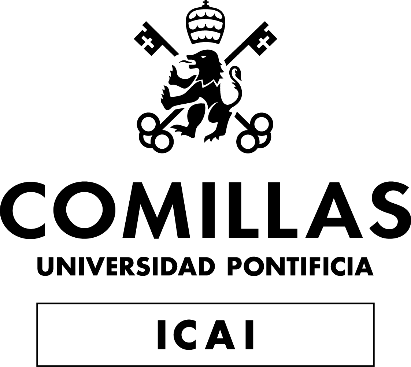
\includegraphics[width=0.35\textwidth]{images/Logo_comillas.png}\\[1cm] 

    {\Huge \textbf{GRADO EN INGENIER\'IA}}\\[0.3cm]
    {\Huge \textbf{MATEM\'ATICA E INTELIGENCIA}}\\[0.5cm]
    {\Huge \textbf{ARTIFICIAL}}\\[1.5cm]

    {\Huge \textbf{TRABAJO FIN DE GRADO}}\\[1.3cm]

    {\huge \projectTitle}\\[0.5cm]

    \vspace{20mm}

    \textbf{Autor: \Author}\\[1.0cm]
    \textbf{Director: \Director}\\

    \raisebox{-2cm}[0cm][0cm]{\large Madrid, \MonthToSubmit \EndYear}

    \vfill
\end{titlepage}
}

\newcommand{\sectionnotoc}[1]{%
    \refstepcounter{section}%
    \section*{\thesection\quad #1}%
}

\newcommand{\resetcounters}{
    \setcounter{section}{0}
    \setcounter{subsection}{0}
    \setcounter{subsubsection}{0}
    \setcounter{figure}{0}
    \setcounter{table}{0}
    \setcounter{equation}{0}
    \setcounter{footnote}{0}
}

%%%%%%%%%%%%%%%%%%%%%%%%%%%%%%%%%%%%%%%%%%%%%%%%%%%%%%%%%%%%%%%%%%%%%%%%%%%%%%%%%%%%%%%%%%%
%%%%%%%%%%%%%%%%%%%%%%%%%%%%%%%%%%%%%%%%%%%%%%%%%%%%%%%%%%%%%%%%%%%%%%%%%%%%%%%%%%%%%%%%%%%

\geometry{top=2.5cm, bottom=4cm, left=2.5cm, right=2.5cm}

\begin{document}

\selectlanguage{spanish}

\ComillasTitlePage

\setlength{\headheight}{2cm}

% Configuraci\'on del encabezado
\pagestyle{fancy}
\fancyhf{}

\fancyhead[L]{
\includegraphics[width=2cm]{images/Color_logo_comillas.png}} 

\fancyhead[C]{
    \textbf{UNIVERSIDAD PONTIFICIA COMILLAS}\\
    Escuela T\'ecnica Superior de Ingenier\'ia (ICAI)\\
    Grado en Ingenier\'ia Matem\'atica e Inteligencia Artificial
}

\fancyfoot[C]{\thepage}

\blankpage

\subfile{Anexo_I_spanish.tex}

\newpage

\ComillasTitlePage

\pagenumbering{roman}
\setcounter{page}{1}

%%%%%%%%%%%%%%%%%%%%%%%%%%%%%%%%%%%%%%%%%%%%%%%%%%%%%%%%%%%%%%%%%%%%%%%%%%%%%%%%%%%%%%%%%%%
%% RESUMEN EJECUTIVO IN SPANISH
%%%%%%%%%%%%%%%%%%%%%%%%%%%%%%%%%%%%%%%%%%%%%%%%%%%%%%%%%%%%%%%%%%%%%%%%%%%%%%%%%%%%%%%%%%%

\captionsetup[figure]{list=false}
\captionsetup[table]{list=false}

\begin{otherlanguage}{spanish}

{\large \MakeUppercase{\projectTitle}}
\vspace{3mm}

\textbf{Autor: \Author}

Director: \Director

\section*{Resumen}

Este trabajo diseña y construye un simulador multiagente de propagación de narrativas sobre redes complejas para medir la \emph{resistencia cognitiva} de una población frente a un ataque informativo. El simulador combina topologías libre de escala y mundo pequeño con un modelo de agente de umbral lineal, y ejecuta un barrido experimental OFAT (One Factor At a Time) de 2000 corridas con 50 réplicas Monte Carlo. Los resultados muestran que la ganancia de persuasión $\gamma$ y la probabilidad de reenvío son los factores más determinantes de la vulnerabilidad, y que la red libre de escala es significativamente más vulnerable que la de mundo pequeño.

\textbf{Palabras clave}: guerra cognitiva; modelado basado en agentes; resiliencia cognitiva; redes complejas; propagación de narrativas; libre de escala; mundo pequeño.

\section*{Resumen ejecutivo}

\sectionnotoc{Introducci\'on}

La desinformación en redes sociales ha dejado de ser un fenómeno marginal para convertirse en un instrumento de \emph{guerra cognitiva}: el empleo deliberado de mensajes para alterar la percepción, la creencia y la decisión de una población objetivo. La OTAN reconoce formalmente la mente humana como dominio operativo y define la superioridad cognitiva como la capacidad de percibir y actuar sobre el entorno con mayor eficacia que el adversario. La información falsa se propaga hasta seis veces más rápido que la veraz, y los ataques se amplifican mediante la estructura de las plataformas digitales, cuyas redes libre de escala concentran la influencia en un pequeño número de \emph{hubs}.

Pese a la creciente literatura doctrinal, existe un vacío metodológico: no se dispone de un banco de pruebas abierto, cuantitativo y reproducible que permita medir cómo la \emph{resistencia cognitiva} de una población depende de (i) la topología de la red social y (ii) los parámetros de la campaña informativa. Este trabajo cubre ese vacío.

\sectionnotoc{Objetivos}

El objetivo principal es diseñar y construir un simulador multiagente de propagación de narrativas que permita medir la resistencia cognitiva de una población ante distintas condiciones de ataque. Los objetivos secundarios son: (O1) formalizar la sociedad como grafo en sus variantes libre de escala (capa digital) y mundo pequeño (capa analógica); (O2) implementar un agente de umbral lineal con heterogeneidad cognitiva; y (O3) ejecutar un barrido experimental OFAT sobre cinco palancas de la narrativa y cuantificar su efecto sobre la resiliencia poblacional.

La pregunta central del trabajo es: \emph{¿qué propiedades de la narrativa y de la red determinan si una población resiste o colapsa ante una campaña de desinformación?}

\sectionnotoc{Descripci\'on del simulador}

El simulador se construye sobre \texttt{Mesa\,3.x} (Python) y \texttt{NetworkX}. El objeto central es el mensaje, formalizado como una tupla de doce campos que incluye veracidad percibida, carga emocional y trazabilidad causal. Cada agente ejecuta el bucle OODA: observa mensajes, actualiza su convicción $c_i$ según la ecuación $c_i \leftarrow c_i + (1-c_i)\cdot\tau\cdot\lambda\cdot\gamma$, y adopta la narrativa cuando $c_i \geq \theta_i$. El umbral $\theta_i$ se muestrea de una distribución bimodal que modela dos subpoblaciones: susceptibles ($\mu_s = 0{,}30$) y resistentes ($\mu_r = 0{,}70$).

\begin{figure}[h!]
    \centering
    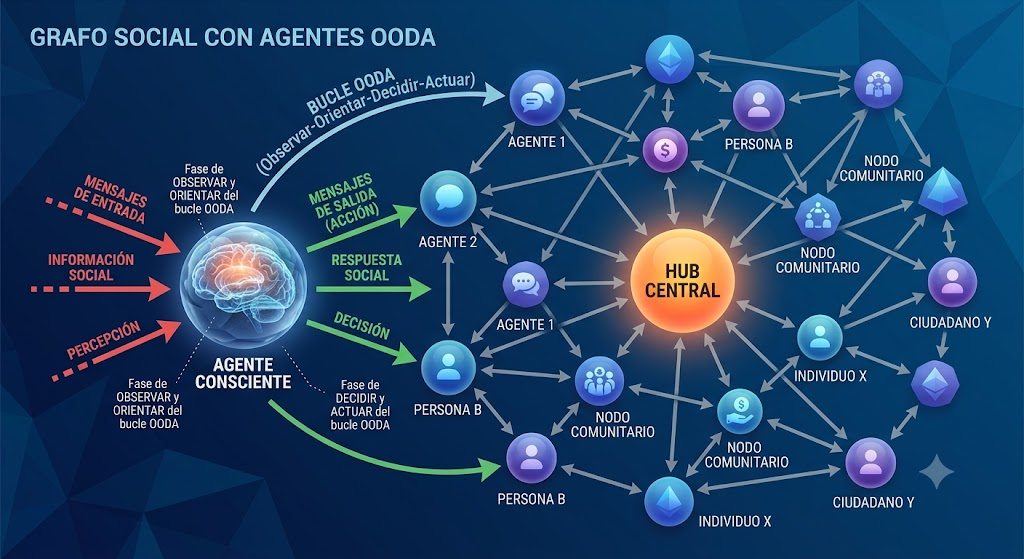
\includegraphics[width=0.90\linewidth]{images/arquitectura_grafo_agentes.jpg}
    \caption{Arquitectura del agente resistente sobre la red social. Un nodo de la red (con cerebro) se expande para mostrar el bucle OODA: \textbf{(1)~Observar} (filtrar mensajes de narrativa del inbox), \textbf{(2)~Orientar} (actualizar convicción $c_i$ y comprobar umbral $\theta_i$) y \textbf{(3)~Decidir/Actuar} (re-emitir narrativa o ruido al grafo).}
    \label{fig:arch-es}
\end{figure}

El diseño experimental sigue la estrategia OFAT: se fija una configuración de referencia y se varía un único factor por experimento sobre dos topologías (libre de escala y mundo pequeño). En total se ejecutan 2000 corridas de simulación con $N = 10\,000$ agentes y 45 pasos de simulación.

\sectionnotoc{Resultados}

La Figura~\ref{fig:arch-es} ilustra la arquitectura del agente y su posición en la red; los resultados cuantitativos del barrido se detallan en el Capítulo~\ref{sec:results}. En síntesis: Los factores más determinantes de la vulnerabilidad son la \textbf{ganancia de persuasión} $\gamma$ y la \textbf{probabilidad de reenvío} $f$: al pasar $\gamma$ de $0{,}25$ a $0{,}75$, la tasa de ataque aumenta de $0{,}32$ a $0{,}59$ en la red libre de escala y de $0{,}05$ a $0{,}69$ en la red de mundo pequeño. La probabilidad de reenvío muestra un patrón similar: $f = 0{,}4$ casi triplica la penetración respecto a $f = 0{,}1$.

La \textbf{estrategia de siembra} es el factor más asimétrico: en la red libre de escala, sembrar en \emph{hubs} produce una tasa de ataque de $0{,}52 \pm 0{,}05$ frente a $0{,}16 \pm 0{,}12$ con siembra aleatoria (brecha de 24 puntos porcentuales). En la red de mundo pequeño la asimetría es menor ($0{,}25$ vs $0{,}17$), lo que refleja la ausencia de \emph{hubs} de alto grado.

La \textbf{topología} es el factor estructural dominante: bajo condiciones de referencia, la resiliencia de la red de mundo pequeño ($R = 0{,}75$) es significativamente superior a la de la red libre de escala ($R = 0{,}48$). La velocidad de propagación también difiere: el tiempo de penetración $t_{50}$ es de $\approx 15$ pasos en la red libre de escala frente a $\approx 32$ en la de mundo pequeño, mostrando que los \emph{hubs} aceleran la cascada de adopción.

\sectionnotoc{Conclusiones}

El simulador demuestra que la resiliencia cognitiva de una población es una propiedad emergente sensible a factores controlables por el atacante ($\gamma$, $f$, estrategia de semilla) y a propiedades estructurales de la red (topología). Las dos principales aportaciones metodológicas son: (i) un banco de pruebas abierto y reproducible para medir la resistencia cognitiva en función de parámetros de la campaña y de la red, y (ii) un conjunto de métricas operacionales ---tasa de ataque, resiliencia, entropía cognitiva, $t_{50}$--- que trasladan el concepto de superioridad cognitiva de la OTAN a magnitudes medibles sobre una población simulada.

La línea de trabajo futuro más relevante es extender el experimento al agente cognitivo-emocional bayesiano y a redes reales descargadas de SNAP, así como estudiar contramedidas de resiliencia (vacunación topológica, inyección de contra-narrativa) cuantificando su eficacia en el mismo marco experimental.

\end{otherlanguage}

%%%%%%%%%%%%%%%%%%%%%%%%%%%%%%%%%%%%%%%%%%%%%%%%%%%%%%%%%%%%%%%%%%%%%%%%%%%%%%%%%%%%%%%%%%%
%% EXECUTIVE SUMMARY IN ENGLISH
%%%%%%%%%%%%%%%%%%%%%%%%%%%%%%%%%%%%%%%%%%%%%%%%%%%%%%%%%%%%%%%%%%%%%%%%%%%%%%%%%%%%%%%%%%%

\newpage

\resetcounters

\begin{otherlanguage}{english}

{\large \MakeUppercase{\projectTitleEnglish}}
\vspace{3mm}

\textbf{Author: \Author}

Director: \Director

\section*{Abstract}

This work designs and builds a multi-agent simulator of narrative propagation over complex networks to measure the \emph{cognitive resilience} of a population against an information attack. The simulator combines scale-free and small-world topologies with a linear threshold agent model and runs an OFAT (One Factor At a Time) experimental sweep of 2\,000 runs with 50 Monte Carlo replicas. Results show that persuasion gain $\gamma$ and forwarding probability are the strongest drivers of vulnerability, and that scale-free networks are significantly more vulnerable than small-world networks.

\textbf{Keywords}: cognitive warfare; agent-based modelling; cognitive resilience; complex networks; narrative propagation; scale-free; small-world.

\section*{Executive Summary}

\sectionnotoc{Introduction}

Disinformation in social networks has evolved from a marginal phenomenon into an instrument of \emph{cognitive warfare}: the deliberate use of messages to alter the perception, belief and decision-making of a target population. NATO formally recognises the human mind as an operational domain and defines cognitive superiority as the ability to perceive and act on the environment more effectively than the adversary. False information spreads up to six times faster than true information, and attacks are amplified by the structure of digital platforms, whose scale-free networks concentrate influence in a small number of high-degree \emph{hubs}.

Despite a growing doctrinal literature, a methodological gap remains: there is no open, quantitative, reproducible testbed that enables measurement of how \emph{cognitive resilience} depends on (i) the topology of the social network and (ii) the parameters of the information campaign. This work fills that gap.

\sectionnotoc{Objectives}

The primary objective is to design and build a multi-agent simulator of narrative propagation capable of measuring the cognitive resilience of a population under varying attack conditions. Secondary objectives are: (O1) formalise society as a graph in its scale-free (digital layer) and small-world (analogue layer) variants; (O2) implement a linear threshold agent with cognitive heterogeneity; and (O3) execute an OFAT experimental sweep over five narrative levers and quantify their effect on population resilience.

The central research question is: \emph{which properties of the narrative and the network determine whether a population resists or collapses under a disinformation campaign?}

\sectionnotoc{Description of the Simulator}

The simulator is built on \texttt{Mesa\,3.x} (Python) and \texttt{NetworkX}. The central object is the message, formalised as a twelve-field tuple including perceived veracity, emotional load and causal traceability. Each agent executes the OODA loop: it observes messages, updates its conviction $c_i$ according to $c_i \leftarrow c_i + (1-c_i)\cdot\tau\cdot\lambda\cdot\gamma$, and adopts the narrative when $c_i \geq \theta_i$. The threshold $\theta_i$ is sampled from a bimodal distribution modelling two subpopulations: susceptible ($\mu_s = 0.30$) and resistant ($\mu_r = 0.70$).

\begin{figure}[h!]
    \centering
    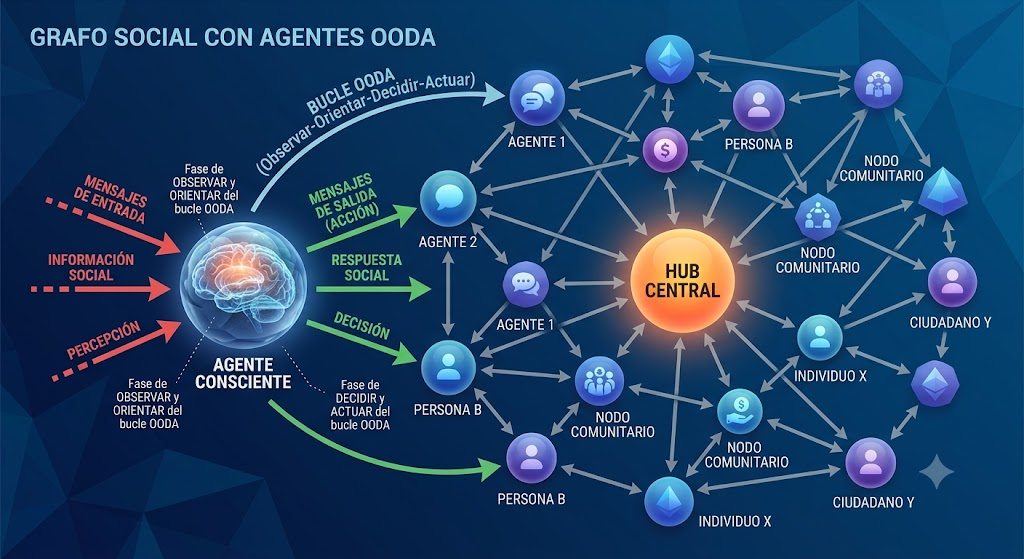
\includegraphics[width=0.90\linewidth]{images/arquitectura_grafo_agentes.jpg}
    \caption{Architecture of the resistant agent on the social network. One node of the network (with a brain) is expanded to show the OODA loop: \textbf{(1)~Observe} (filter narrative messages from inbox), \textbf{(2)~Orient} (update conviction $c_i$ and check threshold $\theta_i$) and \textbf{(3)~Decide/Act} (re-emit narrative or noise to the graph).}
    \label{fig:arch-en}
\end{figure}

The experimental design follows the OFAT strategy: a reference configuration is fixed and a single factor is varied per experiment across two topologies (scale-free and small-world). In total, 2\,000 simulation runs are executed with $N = 10\,000$ agents and 45 simulation steps.

\sectionnotoc{Results}

Figure~\ref{fig:arch-en} illustrates the agent architecture and its position in the network; detailed quantitative results of the sweep are in Chapter~\ref{sec:results}. In summary: the strongest drivers of vulnerability are \textbf{persuasion gain} $\gamma$ and \textbf{forwarding probability} $f$: raising $\gamma$ from $0.25$ to $0.75$ increases the attack rate from $0.32$ to $0.59$ on scale-free networks and from $0.05$ to $0.69$ on small-world networks. The forwarding probability shows a similar pattern: $f = 0.4$ nearly triples penetration relative to $f = 0.1$.

\textbf{Seeding strategy} is the most asymmetric factor: on scale-free networks, hub seeding produces an attack rate of $0.52 \pm 0.05$ vs $0.16 \pm 0.12$ for random seeding (a 24 percentage-point gap). On small-world networks the asymmetry is smaller ($0.25$ vs $0.17$), reflecting the absence of high-degree hubs.

\textbf{Network topology} is the dominant structural factor: under baseline conditions, the resilience of the small-world network ($R = 0.75$) is significantly higher than that of the scale-free network ($R = 0.48$). Propagation speed also differs: the half-adoption time $t_{50}$ is $\approx 15$ steps on scale-free vs $\approx 32$ steps on small-world, showing that hubs accelerate the adoption cascade.

\sectionnotoc{Conclusions}

The simulator demonstrates that the cognitive resilience of a population is an emergent property sensitive to parameters controllable by the attacker ($\gamma$, $f$, seeding strategy) and to structural properties of the network (topology). The two main methodological contributions are: (i) an open, reproducible testbed for measuring cognitive resilience as a function of campaign and network parameters, and (ii) a set of operational metrics---attack rate, resilience, cognitive entropy, $t_{50}$---that translate NATO's concept of cognitive superiority into measurable quantities over a simulated population.

The most relevant direction for future work is to extend the experiments to the Bayesian cognitive-emotional agent and to real-world networks from SNAP, and to study resilience countermeasures (topological vaccination, counter-narrative injection) by quantifying their effectiveness within the same experimental framework.

\end{otherlanguage}

\newpage

\resetcounters

\captionsetup[figure]{list=true}
\captionsetup[table]{list=true}

\pagenumbering{arabic}
\setcounter{page}{1}

\tableofcontents
\thispagestyle{fancy}
\newpage
\setcounter{page}{1}
\fancyfoot[C]{
    \begin{center}
        \thepage
    \end{center}
} 
\renewcommand{\footrulewidth}{0.4pt}
\setlength{\footskip}{0.8cm}

\newpage
\selectlanguage{spanish}

\phantomsection
\listoffigures

\newpage

\phantomsection
\listoftables

\newpage

%%%%%%%%%%%%%%%%%%%%%%%%%%%%%%%%%%%%%%%%%%%%%%%%%%%%%%%%
%%%% Introducci\'on %%%%%%%%%%%%%%%%%%%%%%%%%%%%%%%%%%%%%%
%%%%%%%%%%%%%%%%%%%%%%%%%%%%%%%%%%%%%%%%%%%%%%%%%%%%%%%%


\begin{refsection}[ref_tfg.bib]
\section{Introducci\'on}

La met\'afora de la \emph{aldea global} acu\~nada por McLuhan \cite{McLuhan1964} anticip\'o una humanidad reconectada por los medios electr\'onicos en un \'unico espacio de comunicaci\'on instant\'anea. Las redes sociales digitales han llevado esa intuici\'on al extremo: hoy dos personas cualesquiera est\'an separadas, en promedio, por menos de cuatro intermediarios \cite{Backstrom2012}. Esta hiperconexi\'on, motor de oportunidades sin precedentes, es tambi\'en una superficie de ataque. La informaci\'on falsa se difunde m\'as lejos, m\'as r\'apido y a m\'as personas que la veraz \cite{Vosoughi2018}, y la mediaci\'on algor\'itmica de las plataformas favorece la formaci\'on de c\'amaras de eco y la polarizaci\'on de la opini\'on p\'ublica \cite{DelVicario2016}.

En este contexto ha emergido la \emph{guerra cognitiva} (\emph{cognitive warfare}) como dominio operativo reconocido formalmente por la OTAN, que la define como la lucha por la \emph{superioridad cognitiva} \cite{NATOChiefScientist2025}. A diferencia de la guerra convencional, su terreno no es geogr\'afico sino mental: \emph{el mensaje es la munici\'on y el blanco es la mente} \cite{Hoffman2025}. El objetivo de este cap\'itulo es introducir el problema, justificar por qu\'e debe abordarse y describir la aportaci\'on del trabajo.

\subsection{Motivaci\'on}

La literatura sobre guerra cognitiva ha crecido de forma acelerada entre 2020 y 2026, pero lo ha hecho de manera marcadamente asim\'etrica: es abundante en lo conceptual y doctrinal, y escasa en herramientas \emph{abiertas, cuantitativas y reproducibles} que permitan estudiar el fen\'omeno de forma experimental \cite{DeppeSchaal2024}. La mayor parte de las capacidades operativas, tanto ofensivas como defensivas, permanece clasificada.

Existe, por tanto, un vac\'io metodol\'ogico: no se dispone de un banco de pruebas que permita \emph{medir} c\'omo una poblaci\'on absorbe o resiste la propagaci\'on de una narrativa en funci\'on de (i) la topolog\'ia de la red social que la sostiene y (ii) la psicolog\'ia de los individuos que la componen. Cubrir ese vac\'io —aunque sea parcialmente, sobre un modelo simplificado pero matem\'aticamente fundamentado— es lo que motiva este proyecto, pues habilita el estudio sistem\'atico de la \emph{resiliencia cognitiva} como propiedad emergente y medible de un sistema social.

\subsection{Objetivos}

El objetivo principal de este Trabajo Fin de Grado es:

\begin{itemize}
    \item \textbf{Objetivo principal.} Dise\~nar y construir un simulador multiagente de propagaci\'on de narrativas sobre redes complejas que permita medir la \emph{resistencia cognitiva} de una poblaci\'on frente a un ataque informativo.
\end{itemize}

Para alcanzarlo se definen tres objetivos secundarios:

\begin{itemize}
    \item \textbf{O1.} Formalizar matem\'aticamente la sociedad como un grafo en sus tres registros —aleatorio sint\'etico, multicapa anal\'ogico-digital y real— y caracterizar sus propiedades estructurales.
    \item \textbf{O2.} Formalizar tres modelos de agente de complejidad creciente (reactivo estoc\'astico, resistente por umbral y cognitivo-emocional) y situarlos en la literatura de difusi\'on y contagio social.
    \item \textbf{O3.} Implementar un subconjunto representativo (red libre de escala con agente resistente), definir m\'etricas de resistencia poblacional e individual, y dejar establecido el dise\~no experimental para su evaluaci\'on.
\end{itemize}

\subsection{Estructura del trabajo}

El resto de la memoria se organiza como sigue. 

El Cap\'itulo~\ref{sec:related} (Estado del arte) revisa de forma sint\'etica los trabajos de referencia en guerra cognitiva, modelado de redes complejas y din\'amicas de contagio social. 

El Cap\'itulo~\ref{sec:methodology} (Metodolog\'ia) desarrolla en detalle el marco te\'orico empleado —el mensaje y el bucle OODA, los modelos de grafo y los modelos de agente—, el dise\~no de la soluci\'on programada y su implementaci\'on. 

El Cap\'itulo~\ref{sec:results} (Resultados) describe las m\'etricas y los experimentos previstos. 

Finalmente, el Cap\'itulo~\ref{sec:conclusion} recoge las conclusiones y las l\'ineas de trabajo futuro.

\newpage

%%%%%%%%%%%%%%%%%%%%%%%%%%%%%%%%%%%%%%%%%%%%%%%%%%%%%%%%
%%%% Trabajos relacionados %%%%%%%%%%%%%%%%%%%%%%%%%%%%%
%%%%%%%%%%%%%%%%%%%%%%%%%%%%%%%%%%%%%%%%%%%%%%%%%%%%%%%%
\section{Estado del arte}\label{sec:related}

Este cap\'itulo sit\'ua el proyecto en la literatura mediante una selecci\'on breve de trabajos de referencia en los tres ejes que confluyen en \'el: la guerra cognitiva, el modelado de la sociedad como red compleja y las din\'amicas de contagio y comportamiento colectivo. El desarrollo formal de los modelos se reserva para la metodolog\'ia (Cap\'itulo~\ref{sec:methodology}).

\subsection{Guerra cognitiva}

El documento fundacional de du Cluzel \cite{DuCluzel2021}, elaborado para el Innovation Hub del Mando Aliado de Transformaci\'on de la OTAN, introdujo la definici\'on hoy can\'onica de guerra cognitiva: el arte de emplear tecnolog\'ias para alterar la cognici\'on de objetivos humanos, a menudo sin su conocimiento ni consentimiento. El informe anticip\'o la convergencia de las nano, bio, info y cogno-tecnolog\'ias (NBIC) como multiplicador de la amenaza y advirti\'o de la progresiva armamentizaci\'on de la neurociencia. Su aportaci\'on m\'as duradera es elevar la mente humana a la categor\'ia de dominio operativo, m\'as all\'a de los cinco dominios cl\'asicos (tierra, mar, aire, espacio y ciberespacio).

Deppe y Schaal \cite{DeppeSchaal2024} realizan el primer an\'alisis conceptual acad\'emico del concepto exploratorio de guerra cognitiva del Mando Aliado de Transformaci\'on. Los autores, desde la Universidad de la Bundeswehr, examinan cr\'iticamente la coherencia interna del concepto, delimitan sus fronteras respecto a nociones vecinas (operaciones de informaci\'on, operaciones psicol\'ogicas) y tienden un puente entre la investigaci\'on militar y la civil. Su revisi\'on confirma la asimetr\'ia que motiva este trabajo: la literatura es abundante en lo conceptual y doctrinal, pero escasa en instrumentos emp\'iricos y cuantitativos de medici\'on.

Hoffman \cite{Hoffman2025} ofrece una revisi\'on exhaustiva de la literatura occidental y china sobre el fen\'omeno, fruto de m\'as de cuatro d\'ecadas de experiencia en el Departamento de Defensa estadounidense. Propone una definici\'on refinada centrada en mensajes dirigidos y m\'etodos no violentos contra decisores —civiles o militares— o contra la poblaci\'on general de un Estado objetivo, sintetizada en la m\'axima de que \emph{el mensaje es la munici\'on y el blanco es la mente}. Analiza adem\'as las \emph{Cognitive Domain Operations} del Ej\'ercito Popular de Liberaci\'on chino y el control reflexivo ruso como tradiciones doctrinales paralelas a la occidental.

El informe del Cient\'ifico Jefe de la OTAN \cite{NATOChiefScientist2025} constituye el marco p\'ublico m\'as riguroso publicado hasta la fecha. Define la guerra cognitiva como la lucha por la \emph{superioridad cognitiva} y articula tres funciones operativas: \emph{degradar} las capacidades cognitivas del adversario, \emph{mejorar} las propias y \emph{resistir} los ataques cognitivos. Documenta asimismo el ecosistema investigador de la Alianza —una veintena de actividades de investigaci\'on con m\'as de doscientos expertos de veintis\'eis naciones— y vincula la amenaza a la convergencia NBIC. Es precisamente la tercera funci\'on, la resiliencia, la que el presente trabajo operacionaliza en forma de m\'etricas medibles sobre una poblaci\'on simulada.

Rushing, Hersch y Xu \cite{RushingHerschXu2026} proponen la primera formalizaci\'on unificada de la guerra cognitiva: un marco de interacci\'on atacante--defensor anclado en el bucle OODA (\emph{Observe--Orient--Decide--Act}) y un conjunto de atributos medibles de superioridad cognitiva, ilustrados mediante un caso de estudio. Su contribuci\'on central para este trabajo es conceptual: tratar la cognici\'on colectiva como un sistema observable, atacable y, por tanto, simulable. El bucle OODA de este marco es el que estructura el ciclo de emisi\'on y recepci\'on de mensajes del simulador (Cap\'itulo~\ref{sec:methodology}).

Por \'ultimo, Langlois-Berthelot y Gaie \cite{PolytechniqueCNA2026} sintetizan siete a\~nos de investigaci\'on c\'ivico-militar francesa en el concepto de \emph{Cognitive Net Assessment} (CNA), una adaptaci\'on a la esfera perceptiva del \emph{Net Assessment} del Pent\'agono. El CNA se articula sobre tres ejes cuantificables —sobrecarga decisional, colapso cognitivo y entrop\'ia cognitiva— y documenta el paso de la guerra cognitiva de un estadio artesanal a otro de producci\'on masiva impulsado por la inteligencia artificial generativa. De este marco toma el presente trabajo la entrop\'ia cognitiva como m\'etrica de la diversidad de creencias de la poblaci\'on.

\subsection{Modelado de la sociedad como red compleja}

La representaci\'on de una sociedad como grafo precede en d\'ecadas a la f\'isica de redes complejas y tiene su origen en el \emph{An\'alisis de Redes Sociales} (SNA, \emph{Social Network Analysis}). Moreno \cite{Moreno1934} fund\'o la sociometr\'ia dibujando ya en 1934 \emph{sociogramas} en los que las personas son puntos y sus relaciones, l\'ineas; sobre esa base, las escuelas sociol\'ogicas de las d\'ecadas de 1960 a 1980 consolidaron el SNA como disciplina cuantitativa. Granovetter \cite{Granovetter1973} aport\'o uno de sus resultados m\'as influyentes, la \emph{fuerza de los lazos d\'ebiles}: son los v\'inculos casuales, y no los \'intimos, los que conectan comunidades densas entre s\'i y vehiculan la informaci\'on nueva. El corpus metodol\'ogico del SNA qued\'o sistematizado en el manual de Wasserman y Faust \cite{WassermanFaust1994}, que canoniza las m\'etricas estructurales empleadas en este trabajo: centralidad, cohesi\'on, transitividad y detecci\'on de subgrupos.

La caracterizaci\'on estad\'istica moderna de las redes complejas est\'a sintetizada en el art\'iculo de revisi\'on de Albert y Barab\'asi \cite{AlbertBarabasi2002}. El trabajo unifica los hallazgos emp\'iricos sobre redes reales —distribuciones de grado heterog\'eneas, alto agrupamiento, di\'ametros cortos— y los confronta con los modelos generativos disponibles, demostrando que las redes reales se apartan sistem\'aticamente del paradigma puramente aleatorio. De \'el se toma el aparato formal (distribuci\'on de grado, coeficiente de agrupamiento, longitud media de camino) con el que la metodolog\'ia caracteriza los grafos del simulador.

El modelo de Erd\H{o}s--R\'enyi \cite{ErdosRenyi1960} es el punto de partida de la teor\'ia de grafos aleatorios: cada par de nodos se conecta de forma independiente con probabilidad fija, lo que produce una distribuci\'on de grado de tipo Poisson y permite derivar anal\'iticamente fen\'omenos como la emergencia de la componente gigante. Aunque carece de agrupamiento y de \emph{hubs} —y es por tanto poco realista como modelo de sociedad—, su tratabilidad matem\'atica lo convierte en el \emph{baseline} de referencia frente al que contrastar cualquier topolog\'ia m\'as estructurada.

Watts y Strogatz \cite{WattsStrogatz1998} introdujeron el modelo de \emph{mundo peque\~no} mediante un mecanismo de recableado aleatorio de una ret\'icula regular: basta recablear una peque\~na fracci\'on de aristas para que el di\'ametro de la red colapse mientras el agrupamiento local permanece alto. Esta combinaci\'on —tr\'iadas cerradas y caminos cortos— es exactamente la observada en las redes de relaciones cara a cara, por lo que en este trabajo dicho modelo representa la capa \emph{anal\'ogica} de la sociedad.

Barab\'asi y Albert \cite{BarabasiAlbert1999} mostraron que el crecimiento de la red unido al \emph{enganche preferencial} —los nodos nuevos tienden a conectarse a los ya populares— genera redes \emph{libres de escala} cuya distribuci\'on de grado sigue una ley de potencias. Estas redes exhiben \emph{hubs} que concentran gran parte de la conectividad, lo que las hace robustas frente a fallos aleatorios pero muy vulnerables frente a ataques dirigidos. Esta propiedad, caracter\'istica de las plataformas digitales, fundamenta el experimento de siembra en \emph{hubs} del Cap\'itulo~\ref{sec:results}.

En el plano de las restricciones cognitivas, Dunbar \cite{Dunbar1992} estableci\'o, a partir de la correlaci\'on entre el tama\~no del neoc\'ortex y el de los grupos sociales en primates, que el ser humano puede mantener en torno a 150 relaciones estables y rec\'iprocas. Este l\'imite explica por qu\'e la red anal\'ogica presenta una distribuci\'on de grado acotada, en contraste con las colas pesadas de las plataformas digitales, donde el coste marginal de a\~nadir un v\'inculo es pr\'acticamente nulo.

En el extremo emp\'irico de la escala digital, Backstrom y colaboradores \cite{Backstrom2012} midieron el grafo completo de Facebook —m\'as de 700 millones de usuarios— y obtuvieron una distancia media de 3,74 saltos entre dos personas cualesquiera, muy por debajo de los seis grados cl\'asicos de Milgram. El resultado evidencia la compresi\'on de distancias que las plataformas introducen en la sociedad y justifica la velocidad con que una narrativa puede alcanzar a toda una poblaci\'on conectada.

Finalmente, cuando las dimensiones anal\'ogica y digital coexisten, el formalismo adecuado es el de las \emph{redes multicapa} sistematizado por Kivel\"a y colaboradores \cite{Kivela2014}. Su revisi\'on unifica la notaci\'on del campo y demuestra que agregar las capas en un \'unico grafo destruye informaci\'on estructural y distorsiona m\'etricas como la centralidad o la din\'amica de difusi\'on. Este marco es el que adopta el dise\~no multicapa anal\'ogico-digital del simulador.

\subsection{Comportamiento colectivo y cascadas}

La adopci\'on de una idea o conducta no se explica solo por la estructura de la red, sino tambi\'en por la psicolog\'ia de la decisi\'on individual. Granovetter \cite{Granovetter1978} formaliz\'o los \emph{modelos de umbral} para el comportamiento colectivo: un individuo adopta una conducta cuando la fracci\'on de su entorno que ya lo ha hecho supera su umbral particular. Su an\'alisis demostr\'o un resultado contraintuitivo: es la \emph{heterogeneidad} de la distribuci\'on de umbrales —y no su media— la que determina si la acci\'on colectiva se desencadena o se detiene. Este modelo es la base directa del agente resistente implementado en este trabajo.

Watts \cite{Watts2002} traslad\'o los modelos de umbral a redes aleatorias y demostr\'o que las \emph{cascadas globales} son sucesos poco frecuentes pero de tama\~no enorme cuando ocurren, delimitados por una \emph{ventana de cascada} en el espacio de par\'ametros: si la red es demasiado dispersa la propagaci\'on muere por falta de conectividad, y si es demasiado densa los individuos quedan estabilizados por sus muchos vecinos. La existencia de este punto de inflexi\'on motiva la curva dosis--respuesta del dise\~no experimental del Cap\'itulo~\ref{sec:results}.

Centola y Macy \cite{CentolaMacy2007} introdujeron la distinci\'on entre contagio \emph{simple} y \emph{complejo}. En el contagio simple —propio de enfermedades o de informaci\'on trivial— basta un \'unico contacto para transmitir; en el complejo —propio de creencias, normas y conductas costosas— el individuo requiere refuerzo social desde m\'ultiples fuentes independientes. Los autores muestran que los lazos largos, decisivos para el contagio simple, pueden ser in\'utiles para el complejo. Esta distinci\'on justifica el uso de modelos de umbral, en lugar de modelos puramente epid\'emicos, para representar la adopci\'on de narrativas.

Kempe, Kleinberg y Tardos \cite{KempeKleinbergTardos2003} formularon la \emph{maximizaci\'on de la influencia} como problema algor\'itmico: elegir el conjunto de nodos semilla que maximiza la difusi\'on esperada. Demostraron que el problema es NP-duro pero que, por la submodularidad de la funci\'on de influencia, un algoritmo voraz garantiza una aproximaci\'on del 63\,\% del \'optimo. Visto desde la \'optica de la guerra cognitiva, este resultado describe formalmente la estrategia \'optima del atacante, y es el contrapunto te\'orico del experimento de siembra dirigida en \emph{hubs}.

Del Vicario y colaboradores \cite{DelVicario2016} analizaron emp\'iricamente la difusi\'on de desinformaci\'on en Facebook comparando noticias cient\'ificas y teor\'ias conspirativas. Encontraron que ambas se propagan dentro de \emph{c\'amaras de eco} —comunidades homog\'eneas y polarizadas— y que la homogeneidad ideol\'ogica del vecindario, m\'as que cualquier atributo del contenido, es el principal predictor de la difusi\'on. El hallazgo conecta la estructura comunitaria de la red con la vulnerabilidad cognitiva de la poblaci\'on.

Por \'ultimo, Vosoughi, Roy y Aral \cite{Vosoughi2018} estudiaron unas 126\,000 cascadas de rumores en Twitter verificadas externamente y concluyeron que la informaci\'on falsa llega m\'as lejos, m\'as r\'apido y a m\'as personas que la veraz, y que son los humanos —no los \emph{bots}— quienes la amplifican, atra\'idos por su mayor novedad y por las emociones que suscita. Este resultado respalda la decisi\'on de dotar al objeto mensaje del simulador de una dimensi\'on emocional expl\'icita.

\subsection{Vac\'io identificado}

Pese a la solidez de cada eje por separado, no se ha encontrado un simulador abierto que integre simult\'aneamente una topolog\'ia social realista con confianza diferenciada por capa, un agente cognitivo dotado de umbral de adopci\'on heterog\'eneo, y m\'etricas expl\'icitas de resistencia cognitiva. Cubrir esa intersecci\'on es la aportaci\'on metodol\'ogica de este trabajo.

\newpage


%%%%%%%%%%%%%%%%%%%%%%%%%%%%%%%%%%%%%%%%%%%%%%%%%%%%%%%%
%%%% Metodolog\'ia %%%%%%%%%%%%%%%%%%%%%%%%%%%%%%%%%%%%%%%
%%%%%%%%%%%%%%%%%%%%%%%%%%%%%%%%%%%%%%%%%%%%%%%%%%%%%%%%
\section{Metodolog\'ia}\label{sec:methodology}

Este cap\'itulo desarrolla, en primer lugar, el marco te\'orico que da soporte al simulador —el objeto \emph{mensaje} y el bucle OODA, los modelos de grafo y los modelos de agente—; a continuaci\'on describe el dise\~no de la soluci\'on efectivamente llevada a programaci\'on; y finalmente detalla su implementaci\'on, arquitectura de c\'odigo y reproducibilidad.

\subsection{Marco te\'orico desarrollado}\label{sec:marco}

\subsubsection{Guerra cognitiva: del concepto al modelo operable}
La guerra cognitiva no es una disciplina nueva, pero su formalización operativa como objeto de modelado computacional sí lo es.
Antes de entrar en el modelo, conviene situar el concepto frente a los dos términos con los que a menudo se confunde: las \emph{operaciones psicológicas} (PSYOPS) y las \emph{operaciones de influencia} \cite{RushingHerschXu2026, DeppeSchaal2024}.

Las \textbf{PSYOPS} son acciones comunicativas planificadas y dirigidas a públicos objetivo concretos para modificar actitudes o conductas a corto plazo: históricamente vinculadas a contextos de combate, operan sobre el \emph{contenido} de una creencia específica.
Las \textbf{operaciones de influencia} son más amplias: combinan PSYOPS, medios encubiertos y gestión del entorno informativo para afectar percepciones y procesos decisorios de actores identificados.
La \textbf{guerra cognitiva} eleva el nivel de ambición: su objetivo no es cambiar una creencia concreta, sino reconfigurar la \emph{arquitectura perceptual} del adversario de forma duradera ---los mecanismos mediante los que observa, interpreta y decide sobre cualquier información futura.
Dicho de otro modo: las PSYOPS atacan conclusiones; las operaciones de influencia atacan el entorno informativo; la guerra cognitiva ataca el proceso de razonamiento mismo.

En este marco, el campo de batalla no es territorial sino mental: lo que se disputa es la \emph{superioridad cognitiva}, definida por la OTAN como la capacidad de un actor para percibir, comprender y actuar sobre el entorno con mayor eficacia que sus adversarios \cite{NATOChiefScientist2025}.

\paragraph{Objetivos, capacidades y asimetría de costes.}
El marco de Rushing et al.\ \cite{RushingHerschXu2026} estructura simétricamente los roles de atacante y defensor en cada fase del bucle OODA (Figura~\ref{fig:ooda}).

El \textbf{atacante} opera con alta asimetría de costes a su favor: produce y distribuye narrativas a coste marginal casi nulo aprovechando plataformas digitales e IA generativa.
Sus \emph{objetivos de efecto} son cuatro: (i)~\textbf{efectos de observación} ---saturar o sesgar qué información recibe el objetivo---; (ii)~\textbf{efectos de orientación} ---distorsionar el sensemaking mediante encuadres, cebado emocional o narrativas adversariales---; (iii)~\textbf{efectos de decisión} ---inducir indecisión, sobreconfianza o dependencia de atajos cognitivos---; y (iv)~\textbf{efectos de acción} ---provocar acciones prematuras o desalineadas.
Sus \emph{capacidades habilitadoras} son: acceso y distribución, ingeniería de contenidos y narrativas, amplificación y optimización, y adaptación continua.

El \textbf{defensor} actúa en sentido inverso: preservar la calidad de cada fase del bucle bajo presión adversarial.
Sus \emph{funciones de protección} son simétricas a los efectos del atacante: protección de la observación, protección de la orientación, protección de la decisión y protección de la acción.
Sus \emph{capacidades habilitadoras} son: detección y evaluación, resiliencia cognitiva, respuesta y mitigación, y aprendizaje adaptativo.
La asimetría estructural es desfavorable al defensor: el coste marginal de verificar un mensaje es órdenes de magnitud mayor que el de producirlo, y la latencia de respuesta ---verificación, contra-narrativa, moderación--- supera con creces la del ataque inicial.

\begin{figure}[h!]
\centering
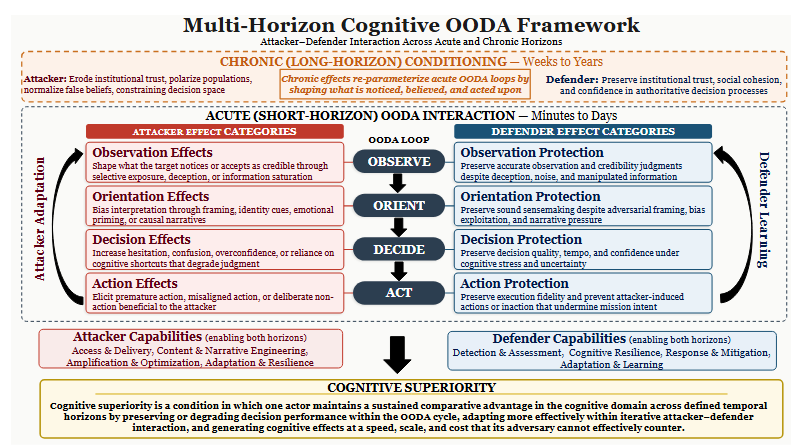
\includegraphics[width=0.95\linewidth]{images/guerra_cognitiva_OODA.png}
\caption{Marco OODA multi-horizonte de la guerra cognitiva \cite{RushingHerschXu2026}. El bucle OODA central articula los efectos del atacante (izquierda) y las protecciones del defensor (derecha) en el horizonte agudo (corto plazo, minutos a días). El horizonte crónico (largo plazo, semanas a años) reconfigura los parámetros del bucle mediante efectos acumulativos sobre creencias y decisiones. La interacción iterativa atacante--defensor determina quién alcanza la superioridad cognitiva.}
\label{fig:ooda}
\end{figure}

Trasladar esta definición a un simulador multiagente requiere fijar la unidad mínima de análisis.
La respuesta que adopta este modelo es inequívoca: \emph{el mensaje es la munición; el blanco, la mente} \cite{Hoffman2025}.
Una operación cognitiva es, en esencia, un flujo de mensajes que altera estados cognitivos; por tanto, el objeto central del modelo no es el agente sino el mensaje que circula entre agentes.

\paragraph{Bucle OODA y horizonte temporal.}
El mecanismo que gobierna la conducta de cada agente sigue el bucle \emph{Observe–Orient–Decide–Act} (OODA) en su variante multi-horizonte \cite{RushingHerschXu2026}, que distingue dos escalas temporales con implicaciones cualitativamente distintas.

El \textbf{horizonte corto plazo} abarca minutos, horas o días: corresponde a la fase aguda de una campaña informativa, en la que la narrativa se difunde rápidamente aprovechando la viralidad de los \emph{hubs} y el contagio emocional antes de que los mecanismos de verificación puedan activarse.
En este horizonte dominan la velocidad de penetración ($t_{50}$), el alcance máximo y la amplitud del pico de nuevas conversiones, junto con las métricas de resultado poblacional: la \textbf{tasa de ataque} $a$ ---fracción de la población que adopta la narrativa--- y la \textbf{resiliencia poblacional} $R = 1 - a$.
Los ataques de corto plazo buscan crear hechos consumados: fijar una versión inicial de los eventos que resulte difícil de desalojar una vez instalada.

El \textbf{horizonte largo plazo} abarca semanas, meses o años: corresponde a la consolidación de la narrativa en las estructuras cognitivas de la población y en la arquitectura de la red.
En este horizonte domina la entropía cognitiva $H$, que mide en qué medida la narrativa ha erosionado la diversidad de creencias de forma estructural y duradera.

El experimento de este trabajo opera exclusivamente en el \textbf{horizonte corto plazo}: la simulación corre durante $45$ pasos equivalentes a tres días de actividad a $15$ pasos/día, donde cada paso representa una hora.
En cada paso cada agente puede procesar y emitir múltiples mensajes, capturando la actividad asíncrona característica del tráfico en redes sociales digitales.
La evaluación del horizonte largo plazo ---consolidación estructural de narrativas, erosión de instituciones--- queda como línea de trabajo futuro.

En cada paso de simulación el agente: (i)~\emph{observa} los mensajes acumulados en su bandeja de entrada (\emph{inbox}); (ii)~\emph{se orienta} actualizando su estado interno; (iii)~\emph{decide} si emite un mensaje nuevo o reenvía alguno de los recibidos; y (iv)~\emph{actúa} depositando el mensaje resultante en su buzón de salida (\emph{outbox}).
Para garantizar determinismo y eliminar condiciones de carrera, el simulador divide cada paso en dos sub-fases secuenciales: \textbf{TX} (todos los agentes ejecutan Decide+Act y pueblan sus \emph{outboxes}) y \textbf{RX} (los mensajes se entregan a los \emph{inboxes} de los destinatarios y se registran en las trazas).
Esta separación asegura que ningún agente procesa en el mismo paso un mensaje que otro acaba de generar, reproduciendo la latencia real de cualquier canal de comunicación.

\paragraph{El mensaje como objeto central.}
El objeto central del modelo es el mensaje, formalizado como una tupla inmutable de doce campos:

\begin{equation}
m = (id,\, trace,\, t,\, src,\, tgt,\, \ell,\, M_{od},\, e,\, \lambda,\, v,\, s,\, parent)
\label{eq:mensaje}
\end{equation}

La Tabla~\ref{tab:mensaje} detalla el dominio y el papel de cada variable.
La \emph{capa} $\ell \in \{\text{analógica},\,\text{digital}\}$ determina la función de confianza aplicable y la modalidad por defecto: la capa analógica corresponde a comunicación presencial (cara a cara), mientras que la digital admite cualquier modalidad.
La \emph{modalidad} $M_{od} \subseteq \{\text{texto},\,\text{audio},\,\text{imagen},\,\text{vídeo}\}$ modula la ganancia de impacto perceptual del mensaje: el vídeo tiene el mayor potencial persuasivo, seguido de audio, imagen y texto, en coherencia con la literatura sobre persuasión multimodal.
La \emph{emoción dominante} $e$ se toma del conjunto de las ocho emociones primarias de Plutchik más la etiqueta neutra \cite{Plutchik1980}; su presencia en el mensaje abre la puerta a modelar contagio emocional sin necesidad de una psicología del agente más elaborada.
La \emph{carga emocional} $\lambda \in [0,1]$ cuantifica la intensidad de esa emoción y constituye el principal driver de persuasión del mensaje: un mensaje puede ser falso y aun así persuadir si su carga emocional es elevada.
La \emph{veracidad percibida} $v \in [0,1]$ no modula directamente la persuasión ---el modelo no asume que los agentes evalúan la verdad--- sino que etiqueta el mensaje como \emph{narrativa} (desinformación) cuando $v \leq v_{thr}$, distinguiéndolo del ruido neutro.
Esta elección está respaldada por la evidencia empírica de que las noticias falsas se difunden significativamente más rápido y más lejos que las verdaderas \cite{Vosoughi2018}.
La \emph{saliencia} $s \in [0,1]$ captura la relevancia subjetiva que el receptor atribuye a la fuente; es el mecanismo por el que las fuentes de autoridad percibida ejercen mayor influencia.
Por último, los campos $trace$ y $parent$ implementan la trazabilidad causal: $trace$ agrupa todos los mensajes de una misma campaña y $parent$ apunta al mensaje del que este es reenvío directo, permitiendo reconstruir el árbol de difusión completo para análisis \emph{post hoc}.

\begin{table}[h!]
\centering
\caption{Variables del mensaje $m$ (ecuación~\ref{eq:mensaje}): símbolo, dominio y papel en el modelo.}
\label{tab:mensaje}
\begin{tabular}{@{}l p{4.2cm} p{8cm}@{}}
\toprule
\textbf{Símbolo} & \textbf{Dominio} & \textbf{Papel en el modelo} \\
\midrule
$id$       & UUID                                           & Identificador único del mensaje \\
$trace$    & UUID                                           & Identificador de campaña; agrupa mensajes relacionados \\
$t$        & $\mathbb{N}$                                   & Paso de simulación en que se emite \\
$src$      & $V$ (nodo del grafo)                           & Agente emisor \\
$tgt$      & $V$ (nodo del grafo)                           & Agente receptor \\
$\ell$     & \{analógica, digital\}                         & Capa; determina función de confianza y modalidad por defecto \\
$M_{od}$   & $\mathcal{P}$(\{texto, audio, imagen, vídeo\}) & Modalidad/canal; modula ganancia de impacto perceptual \\
$e$        & Emociones Plutchik $\cup$ \{neutro\}           & Emoción dominante del mensaje \cite{Plutchik1980} \\
$\lambda$  & $[0,1]$                                        & Carga emocional; intensidad de la emoción del mensaje \\
$v$        & $[0,1]$                                        & Veracidad percibida; etiqueta narrativa si $v \leq v_{thr}$ \\
$s$        & $[0,1]$                                        & Saliencia; relevancia subjetiva atribuida al emisor \\
$parent$   & UUID $\cup$ \{\texttt{None}\}                  & Referencia al mensaje origen (trazabilidad causal) \\
\bottomrule
\end{tabular}
\end{table}

La dinámica emergente del modelo nace de la coexistencia de dos \emph{especies} de mensajes con propiedades opuestas.
La \emph{narrativa} se caracteriza por veracidad percibida baja ($v \leq v_{thr}$) y carga emocional alta ($\lambda \approx 1$): es el vector de desinformación que persuade precisamente porque apela a la emoción y no a la evidencia.
El \emph{ruido neutro}, en cambio, presenta veracidad alta y emoción neutra: no persuade, pero mantiene activo el canal de comunicación y proporciona el ruido de fondo sobre el que la narrativa compite.
Su competencia sobre la misma red genera patrones de difusión no lineales que la simulación permite observar y medir.
La métrica que captura el efecto agregado es la \emph{entropía cognitiva} definida en el marco del \emph{Cognitive Net Assessment} \cite{PolytechniqueCNA2026}: una población con creencias distribuidas de forma más uniforme ---mayor entropía--- es más vulnerable a la narrativa, porque ninguna creencia dominante actúa como ancla colectiva.
Esta métrica operacionalizará el concepto de superioridad cognitiva en la fase de análisis de resultados, cerrando el ciclo entre el marco teórico y el diseño computacional del simulador.


\subsubsection{Grafos: la sociedad como red}
%! Subsubsección: Grafos: la sociedad como red
% Cuerpo sin encabezado de sección.

Una red social puede representarse formalmente como un grafo $G = (V, E)$, donde el conjunto de nodos $V$ corresponde a los individuos que participan en el sistema y el conjunto de aristas $E \subseteq V \times V$ representa los vínculos entre ellos. Según la naturaleza de dichos vínculos, el grafo puede ser \emph{no dirigido} (relaciones simétricas de amistad o conocimiento mutuo), \emph{dirigido} (relaciones asimétricas como el seguimiento en redes digitales), \emph{ponderado} (cuando se asigna un valor numérico de confianza o intensidad a cada arista) o \emph{multicapa} (cuando coexisten distintos tipos de red sobre el mismo conjunto de individuos). Esta representación unificada permite aplicar al estudio de la influencia social el aparato matemático de la teoría de grafos y la ciencia de redes \cite{AlbertBarabasi2002}.

\paragraph{Métricas estructurales.}
La caracterización cuantitativa de una red requiere el cálculo de un conjunto de métricas estructurales que el módulo \texttt{compute\_graph\_metrics} del proyecto evalúa sobre cada topología generada. El \emph{grado} $k_i$ de un nodo $i$ es el número de aristas que lo inciden; en redes dirigidas se distinguen el grado de entrada $k_i^{\text{in}}$ y el de salida $k_i^{\text{out}}$. La distribución de grado $P(k)$ describe la fracción de nodos con grado $k$ y constituye la huella estructural más característica de cada modelo de red. El \emph{coeficiente de clustering} $C_i$ mide la densidad de triángulos en el vecindario de $i$, mientras que la \emph{longitud media de camino} $\langle \ell \rangle$ refleja la eficiencia global de la propagación de información a través de la red. Las \emph{centralidades} de intermediación, de vector propio y PageRank cuantifican, respectivamente, el control de flujo, la influencia transitiva y la notoriedad de cada nodo. La \emph{asortatividad} indica si los nodos de grado elevado tienden a conectarse entre sí o con nodos periféricos.

Cuando la distribución de grado sigue una \emph{ley de potencias}, se cumple

\begin{equation}
  P(k) \propto k^{-\gamma},
  \label{eq:powerlaw}
\end{equation}

donde el exponente $\gamma$ se estima mediante el estimador de máxima verosimilitud de Clauset, Shalizi y Newman \cite{Clauset2009}:

\[
  \hat{\gamma} = 1 + n \left[ \sum_{i=1}^{n} \ln\!\left( \frac{k_i}{k_{\min} - \tfrac{1}{2}} \right) \right]^{-1},
\]

con $k_{\min}$ el grado mínimo a partir del cual se ajusta la ley y $n$ el número de nodos con $k_i \geq k_{\min}$. Este estimador es asintóticamente insesgado y se utiliza en el código para caracterizar automáticamente las redes de escala libre generadas.

\paragraph{Topologías implementadas.}
El simulador incorpora tres modelos de red canónicos que sirven de base a todas las configuraciones de experimento.

El modelo de \emph{Erdős–Rényi} $\mathcal{G}(n, p)$ \cite{ErdosRenyi1960} construye el grafo conectando cada par de nodos de forma independiente con probabilidad $p$. El grado de cada nodo sigue una distribución de Poisson con media $\langle k \rangle = (n-1)p$. Esta topología se usa exclusivamente como \emph{baseline} aleatorio: carece de hubs, presenta clustering bajo y no reproduce las heterogeneidades observadas en redes humanas reales.

El modelo \emph{libre de escala} \cite{BarabasiAlbert1999, AlbertBarabasi2002} se basa en el mecanismo de adjunción preferencial: los nodos nuevos se enlazan con mayor probabilidad a nodos ya bien conectados, lo que genera la distribución de grado~\eqref{eq:powerlaw} con exponente $\gamma \in [2, 3]$ y una minoría de nodos con grado excepcional (\emph{hubs}). En el código se utiliza la generalización dirigida de Bollobás et al.\ \cite{Bollobas2003}, implementada mediante \texttt{nx.scale\_free\_graph}, que introduce tres parámetros de mezcla $\alpha + \beta + \gamma = 1$: $\alpha$ controla la probabilidad de añadir un nodo nuevo con arista de entrada, $\beta$ la de añadir una arista entre nodos existentes, y $\gamma$ la de añadir un nodo nuevo con arista de salida; los sesgos $\delta_{\text{in}}$ y $\delta_{\text{out}}$ modulan la preferencia de adjunción. Esta topología modela la \emph{red digital}: la distancia media entre usuarios en Facebook se aproxima a 3{,}5 saltos \cite{Backstrom2012}, confirmando el efecto del mundo pequeño inducido por los hubs.

El modelo de \emph{Watts–Strogatz} \cite{WattsStrogatz1998} parte de un anillo regular donde cada nodo está conectado a sus $k$ vecinos más próximos y, posteriormente, recablea cada arista con probabilidad $p$. Para valores intermedios de $p$ se obtiene simultáneamente un coeficiente de clustering elevado (herencia de la estructura regular) y caminos medios cortos proporcionales a $\log n$ (consecuencia del recableado aleatorio). Esta topología modela la \emph{red analógica}, cuya estructura refleja la organización comunitaria de las relaciones presenciales.

La figura~\ref{fig:pk} compara las distribuciones de grado de los tres modelos en escala logarítmica.

\begin{figure}[h!]
  \centering
  \fbox{\parbox{0.85\linewidth}{\centering\vspace{1.5cm}
    PENDIENTE (figura a generar): Distribuciones de grado $P(k)$ en escala log-log para los tres modelos de red implementados: Erdős–Rényi (distribución de Poisson, caída exponencial), libre de escala (recta de pendiente $-\gamma$, hubs visibles) y Watts–Strogatz (distribución acotada con pico estrecho). Ejes: $\log k$ frente a $\log P(k)$.
    \vspace{1.5cm}}}
  \caption{Distribuciones de grado $P(k)$ en escala log-log para los modelos Erdős–Rényi, libre de escala (Barabási–Albert) y Watts–Strogatz. La recta de pendiente $-\gamma$ en la red libre de escala evidencia el comportamiento de ley de potencias~\eqref{eq:powerlaw}.}
  \label{fig:pk}
\end{figure}

\paragraph{Confianza por capa.}
La confianza entre dos agentes no es homogénea ni estática, sino que depende de la capa de red en la que se establece el vínculo. El módulo \texttt{src/graphs/trust.py} implementa dos modelos diferenciados.

En la \emph{capa analógica}, la confianza se asigna conforme al modelo de Dunbar \cite{Dunbar1992}: la distancia circular entre dos nodos $u$ y $v$ en el anillo de Watts–Strogatz se define como $d = \min(|u - v|,\, n - |u - v|)$, y el valor de confianza se asigna en función de la banda de Dunbar a la que pertenece dicha distancia — núcleo íntimo ($\leq 5$), círculo cercano ($\leq 15$), amigos ($\leq 50$) o conocidos ($\leq 150$) —, de modo que a mayor distancia corresponde menor confianza. Esta graduación reproduce la estructura jerárquica observada empíricamente en las redes de relación humana presencial.

En la \emph{capa digital}, la confianza se modela mediante una distribución log-normal cuya media y varianza dependen de las propiedades estructurales de emisor y receptor:

\begin{equation}
  \tau^{\text{dig}}_{a \to b} = \mathrm{clip}\!\left(\,\mathcal{N}(\mu, \sigma) + 0{,}04 \cdot \min(c_{ab}, 5),\; 0,\; 1\right),
  \label{eq:digital-trust}
\end{equation}

donde $\mu = 1 / (1 + 0{,}005 \cdot k_b^{\text{in}})$, $\sigma = 0{,}05 + 0{,}003 \cdot k_a^{\text{out}}$, $k_b^{\text{in}}$ es el in-grado del receptor $b$, $k_a^{\text{out}}$ el out-grado del emisor $a$, y $c_{ab}$ el número de vecinos comunes entre $a$ y $b$. La interpretación es directa: los hubs con muchos seguidores generan una confianza por contacto decreciente (efecto de \emph{saturación}), mientras que compartir vecinos introduce un pequeño bono de credibilidad basado en el principio de cierre triádico.

\paragraph{Redes multicapa.}
Cuando se desea modelar simultáneamente las interacciones analógicas y digitales de una misma población, el formalismo de redes multicapa \cite{Kivela2014, DeDomenico2013} proporciona el marco apropiado. Una red multicapa se define formalmente como la tupla $\mathcal{M} = (V_\mathcal{M}, E_\mathcal{M}, V, L)$, donde $L = \{L_1, \ldots, L_d\}$ es el conjunto de capas, $V_\mathcal{M} \subseteq V \times L$ el conjunto de nodos-capa y $E_\mathcal{M}$ incluye tanto aristas \emph{intra-capa} (dentro de una misma capa) como aristas \emph{inter-capa} (entre capas).

En el simulador, la clase \texttt{MultiLayerGraph} construye un \texttt{MultiDiGraph} de NetworkX con dos capas: la digital (libre de escala, prioritaria) y la analógica (Watts–Strogatz). Se mantiene el invariante de que ningún par $\{u, v\}$ aparece simultáneamente en ambas capas, evitando duplicidades que distorsionarían la dinámica de propagación. La \emph{participación} de un nodo en las distintas capas se cuantifica mediante el índice

\begin{equation}
  P_i = 1 - \sum_{\ell} \left( \frac{k_{i,\ell}}{k_i} \right)^2,
  \label{eq:participacion}
\end{equation}

donde $k_{i,\ell}$ es el grado del nodo $i$ en la capa $\ell$ y $k_i = \sum_\ell k_{i,\ell}$ su grado total. Un valor $P_i \approx 1$ indica participación equilibrada entre capas, mientras que $P_i \approx 0$ señala que toda la actividad del nodo se concentra en una única capa. Este índice, junto con la correlación de grado entre capas, permite diagnosticar la dualidad analógico-digital de cada agente.

\begin{figure}[h!]
  \centering
  \fbox{\parbox{0.85\linewidth}{\centering\vspace{1.5cm}
    PENDIENTE (figura a generar): Esquema de la red multicapa analógico-digital. Se muestran dos planos paralelos: el superior representa la capa digital (libre de escala, con hubs bien visibles) y el inferior la capa analógica (Watts–Strogatz, estructura de anillo con conexiones locales). Las aristas inter-capa (punteadas verticales) conectan el mismo nodo en ambas capas. El código de colores distingue aristas intra-capa analógica (azul), intra-capa digital (naranja) e inter-capa (gris).
    \vspace{1.5cm}}}
  \caption{Arquitectura de la red multicapa analógico-digital. La capa superior (digital, libre de escala) y la capa inferior (analógica, Watts–Strogatz) comparten el mismo conjunto de nodos $V$; las aristas verticales representan la correspondencia inter-capa.}
  \label{fig:multicapa}
\end{figure}

\paragraph{Redes reales (SNAP).}
Además de las topologías sintéticas, el simulador permite cargar redes empíricas del repositorio SNAP \cite{LeskovecKrevl2014}. Los conjuntos de datos utilizados — redes de ego de Facebook y Twitter, y la red de confianza de Epinions — exhiben los sesgos estructurales característicos de las redes humanas: distribución de grado de cola pesada, alto clustering local y efecto de mundo pequeño. La clase \texttt{SNAPGraph} se encarga de descargar y adaptar estos datos al formato interno del simulador; cuando el grafo original es no dirigido, la orientación de las aristas se asigna de forma probabilística ponderada por el grado de los nodos extremos, aproximando la asimetría típica de las relaciones de influencia en entornos digitales.

\paragraph{Comparativa analógica-digital.}
La tabla~\ref{tab:analog-digital} resume las diferencias estructurales más relevantes entre la red analógica y la digital en el contexto del simulador.

\begin{table}[h!]
  \caption{Comparativa estructural entre la red analógica (Watts–Strogatz) y la red digital (libre de escala) en el simulador.}
  \label{tab:analog-digital}
  \centering
  \begin{tabular}{@{}l p{5cm} p{5.8cm}@{}}
    \toprule
    \textbf{Dimensión} & \textbf{Red analógica} & \textbf{Red digital} \\
    \midrule
    Modelo de base & Watts–Strogatz & Barabási–Albert dirigido \cite{Bollobas2003} \\
    Tamaño de la vecindad & Limitado (bandas de Dunbar \cite{Dunbar1992}) & Ilimitado; hubs con $k \gg \langle k \rangle$ \\
    Coste de vínculo & Alto (tiempo, proximidad física) & Bajo (un clic, coste casi nulo) \\
    Distribución de grado & Acotada, pico estrecho & Ley de potencias, $\gamma \in [2,3]$~\eqref{eq:powerlaw} \\
    Distancia media $\langle \ell \rangle$ & $\mathcal{O}(\log n)$, relativamente larga & Muy corta ($\approx 3{,}5$ saltos \cite{Backstrom2012}) \\
    Coeficiente de clustering & Alto (estructura comunitaria) & Bajo (hubs con vecindarios dispersos) \\
    Mediación algorítmica & Ninguna & Presente (recomendaciones, \emph{trending}) \\
    Confianza por arista & Según bandas de Dunbar & Log-normal modulada por grado~\eqref{eq:digital-trust} \\
    \bottomrule
  \end{tabular}
\end{table}


\subsubsection{Agentes: modelos psicol\'ogicos}
\paragraph{¿Por qué modelos basados en agentes?}

El modelado basado en agentes (ABM, \emph{Agent-Based Modeling}) ofrece ventajas estructurales frente a los enfoques alternativos para simular la propagación de narrativas en redes sociales.

Los modelos de ecuaciones diferenciales ordinarias (ODE), heredados de la epidemiología (modelos SIR, SIS), trabajan con densidades poblacionales homogéneas y asumen que todos los individuos son equivalentes y están en contacto potencial con todos los demás. Esta hipótesis de mezcla homogénea es fundamentalmente incorrecta para redes sociales, donde la estructura de la red ---hubs, comunidades, puentes débiles--- es precisamente el mecanismo que gobierna la difusión \cite{Watts2002,CentolaMacy2007}. Los ABM no imponen dicha homogeneidad: la heterogeneidad emerge de la interacción local entre agentes sobre una topología específica.

Los modelos estadísticos y de aprendizaje automático son potentes para predecir patrones observados, pero no son causales: describen correlaciones entre variables pasadas sin modelar el mecanismo generador. Para el objetivo de este trabajo ---medir cómo la topología y la psicología individual determinan la resiliencia cognitiva--- se requiere un modelo \emph{generativo} que permita intervenir en parámetros individuales y observar el efecto sobre la dinámica colectiva.

Los juegos evolutivos y los modelos de dinámica de opinión (DeGroot, Hegselmann-Krause) capturan la actualización de creencias pero tipicamente asumen homogeneidad de la red, ausencia de contenido emocional en los mensajes, o reglas de actualización simétricas incompatibles con la dirección asimétrica de las plataformas digitales.

El ABM resuelve estas limitaciones con tres propiedades: (i) permite asignar a cada agente un umbral $\theta_i$ individual muestreado de una distribución heterogénea, condición necesaria para observar cascadas no lineales \cite{Granovetter1978}; (ii) sitúa a cada agente en un nodo del grafo y hace que la difusión dependa explícitamente de la estructura de vecindad; y (iii) permite registrar trazas causales de cada mensaje, requisito imprescindible para el análisis \emph{post hoc} de la dinámica de resistencia.

El coste del ABM es computacional: cada réplica simula $N = 5\,000$ agentes durante 45 pasos de simulación, generando decenas de miles de mensajes por corrida. El diseño OFAT con 25 réplicas Monte Carlo y 700 runs totales requiere aproximadamente 30 minutos de CPU con implementación eficiente en Python/Mesa 3.x.

\medskip

El simulador implementa tres modelos de agente de complejidad psicológica creciente.
Su diseño responde a una lógica de control experimental: el modelo más simple actúa como
línea base estadística, el modelo intermedio concentra la potencia explicativa de los
experimentos y el modelo más rico constituye una propuesta teórica para trabajo futuro.
Los tres comparten la misma interfaz de paso de mensaje sobre el grafo, lo que permite
intercambiarlos sin modificar la lógica de la simulación.

\paragraph{Agente estocástico (control nulo).}
La clase \texttt{StochasticAgent} es un agente \emph{reactivo puro}: carece de estado
cognitivo interno y no mantiene ninguna representación de las narrativas que circulan por
la red. Su comportamiento en cada paso de la simulación se reduce a dos acciones
independientes parametrizadas por sendas probabilidades: con probabilidad $p_{\text{fwd}}$
reenvía el último mensaje recibido a un subconjunto aleatorio de sus seguidores en el
grafo, y con probabilidad $p_{\text{fire}}$ genera un mensaje de ruido neutro y lo emite
igualmente a un subconjunto aleatorio. Ambas acciones son independientes en cada paso, de
modo que un agente puede reenviar y generar ruido simultáneamente, solo una de las dos, o
ninguna.

La utilidad de este modelo no es descriptiva sino metodológica. Al eliminar toda
psicología individual, aisla la contribución de la \emph{topología de la red} y del
\emph{azar} en la difusión de contenidos. Cualquier diferencia observada entre las métricas
de este agente y las de los modelos más ricos debe atribuirse, por diferencia, a los
mecanismos cognitivos añadidos en estos últimos. Sin este control nulo sería imposible
separar el efecto estructural del grafo del efecto de los procesos individuales de
resistencia o persuasión.

\paragraph{Agente resistente (umbral lineal cognitivo).}
La clase \texttt{ResistantAgent} es el modelo implementado en los experimentos de esta
memoria. Incorpora un estado interno compuesto por dos escalares: la \emph{convicción}
$c_i \in [0,1]$, que cuantifica en qué medida el agente $i$ ha interiorizado una narrativa
concreta, y el \emph{umbral de resistencia} $\theta_i \in [0,1]$, que marca el nivel de
convicción necesario para que el agente adopte dicha narrativa. El umbral $\theta_i$ se
muestrea de una distribución bimodal que modela dos subpoblaciones —susceptible y
resistente—; su expresión formal se detalla en el diseño de la solución
(ecuación~\ref{eq:theta}).

Un mensaje pertenece a la narrativa rastreada si y solo si su veracidad $v$ satisface
$v \leq v_{\text{thr}}$, donde $v_{\text{thr}}$ es un umbral de veracidad global
configurable. Cuando el agente $i$ recibe un mensaje de la narrativa procedente del
agente $j$, actualiza su convicción según la regla:

\begin{equation}
  c_i \;\leftarrow\; c_i + (1 - c_i)\cdot\tau_{j \to i}\cdot\lambda_m\cdot\gamma,
  \label{eq:conviction}
\end{equation}

donde $\tau_{j \to i}$ es la confianza que el agente $i$ deposita en el emisor $j$ en la
capa del mensaje, $\lambda_m \in [0,1]$ es la \emph{carga emocional} del mensaje y
$\gamma > 0$ es la ganancia de persuasión por exposición. La forma multiplicativa de la
ecuación garantiza que $c_i$ permanezca acotada en $[0,1]$ y que la tasa de incremento
decrezca conforme la convicción se aproxima a la saturación, en línea con el marco del
modelo de umbral lineal de~\cite{KempeKleinbergTardos2003}. El agente adopta la narrativa
en el instante en que $c_i \geq \theta_i$.

La heterogeneidad de los umbrales $\{\theta_i\}$ —no su valor medio— es el factor
determinante en la formación de cascadas de adopción: una distribución concentrada impide
o universaliza la propagación, mientras que la bimodalidad introduce puntos de inflexión
no lineales en la dinámica de difusión~\cite{Granovetter1978,Watts2002}. Adicionalmente,
el hecho de que la adopción requiera exposición reiterada al mismo contenido convierte
este proceso en un \emph{contagio complejo}, cualitativamente distinto de la difusión
simple y más sensible a la estructura de los puentes débiles~\cite{CentolaMacy2007}.

Una vez adoptada la narrativa, el agente no se vuelve pasivo: en cada paso ulterior
re-emite espontáneamente su última narrativa con probabilidad $f$ (período infeccioso
superior a un único paso) y emite ruido neutro con probabilidad $p_{\text{fire}}$. Esta
capacidad de re-emisión autónoma genera un \emph{contagio autosostenido} en el que los
nodos adoptados actúan como fuentes secundarias, amplificando la dinámica de cascada más
allá de la fuente original.

\paragraph{Agente cognitivo-emocional (bayesiano).}
Las clases \texttt{BayesianAgent} y \texttt{EmotionalBrain} forman el modelo teórico más
rico del simulador. No se incluye en los experimentos de esta memoria, pero su diseño
ilustra una dirección de extensión naturalista bien fundamentada. El agente ejecuta el
bucle \emph{OODA} (observar, orientar, decidir, actuar)~\cite{RushingHerschXu2026}, en el
que la fase de orientación está mediada por un \emph{cerebro emocional} vectorial.

El estado interno del cerebro es un vector $\mathbf{e} \in [0,1]^{11}$: las ocho emociones
básicas del modelo de Plutchik~\cite{Plutchik1980} —alegría, confianza, miedo, sorpresa,
tristeza, aversión, ira y anticipación— más tres dimensiones metacognitivas: atención,
credulidad y autoconfianza. Cada agente posee además un vector de \emph{genética}
$\mathbf{g} \in [0,1]^{11}$ que actúa como amplificador estable e individual de la
respuesta emocional, modelando la variabilidad interindividual en sensibilidad afectiva.

Al observar un mensaje, el cerebro actualiza su estado emocional siguiendo el principio
de codificación predictiva y actualización bayesiana de creencias~\cite{Friston2010}:

\begin{equation}
  \Delta = \mathbf{m}_{\text{vec}} \cdot g_{\text{mod}} \cdot \mathbf{g}
           \cdot \mathrm{attn} \cdot \tau \cdot \mathrm{cred} \cdot \mathrm{circ}(t),
  \qquad
  \mathbf{e} \;\leftarrow\; \operatorname{clip}(\mathbf{e} + \Delta,\; 0,\; 1),
  \label{eq:brain}
\end{equation}

donde $\mathbf{m}_{\text{vec}}$ es el vector emocional del mensaje, $g_{\text{mod}}$ un
factor de ganancia por modalidad (texto, imagen, vídeo), $\mathrm{attn}$ la atención
actual del agente, $\tau$ la confianza en el emisor, $\mathrm{cred}$ la credulidad
disposicional y $\mathrm{circ}(t)$ un modulador circadiano. Entre pasos se aplica un
decaimiento exponencial por dimensión
$e_k \leftarrow e_k \cdot 2^{-1/h_{1/2}}$,
donde $h_{1/2}$ es la vida media emocional en pasos de simulación. El modulador circadiano
adopta la forma
\[
  \mathrm{circ}(t) = \mathrm{base} + \mathrm{amp}
  \cdot \cos\!\Bigl(\frac{2\pi(h - h_{\mathrm{pico}})}{24}\Bigr),
\]
con un pico de sugestionabilidad positiva en horas matinales y un pico de afecto negativo
nocturno, en consonancia con los patrones afectivos observados en redes sociales a lo
largo del día~\cite{GolderMacy2011}.

El motivo por el que este modelo no entra en los experimentos es de orden metodológico: el
determinismo y la trazabilidad del agente de umbral bastan para medir la resistencia a la
desinformación de forma reproducible y controlada. El cerebro emocional vectorial introduce
fuentes de no-determinismo adicionales —el decaimiento por dimensión, la modulación
circadiana continua, la interacción multiplicativa de once dimensiones— que, sin un diseño
experimental específicamente orientado a ellas, oscurecerían la atribución causal y
elevarían el coste computacional sin una ganancia proporcional en la validez interna del
experimento.

\begin{figure}[h!]
\centering
\fbox{\parbox{0.85\linewidth}{\centering\vspace{1.5cm}
PENDIENTE (figura a generar): Esquema del cerebro emocional de 11~dimensiones del
\texttt{EmotionalBrain}. Las 8~emociones de Plutchik aparecen en la periferia y las
3~dimensiones metacognitivas (atención, credulidad, autoconfianza) en el centro. Flechas
indican el flujo de actualización al recibir un mensaje: entrada $\mathbf{m}_{\text{vec}}$,
modulación por $\mathbf{g}$, $\tau$, $\mathrm{circ}(t)$, y salida $\mathbf{e}$
actualizado mediante la ecuación~\eqref{eq:brain}.%
\vspace{1.5cm}}}
\caption{Arquitectura del cerebro emocional vectorial del agente cognitivo-emocional.
         El estado interno es un vector de 11~dimensiones actualizado en cada observación
         (ecuación~\eqref{eq:brain}).}
\label{fig:cerebro}
\end{figure}

\begin{figure}[h!]
\centering
\fbox{\parbox{0.85\linewidth}{\centering\vspace{1.5cm}
PENDIENTE (figura a generar): Rueda de emociones de Plutchik~\cite{Plutchik1980} con las
ocho emociones básicas y sus combinaciones diádicas primarias, coloreada según valencia
afectiva (tonos cálidos para emociones positivas, fríos para negativas). Se destacan las
ocho dimensiones adoptadas en el modelo:
\textit{joy, trust, fear, surprise, sadness, disgust, anger, anticipation}.%
\vspace{1.5cm}}}
\caption{Rueda de emociones de Plutchik~\cite{Plutchik1980}. Las ocho emociones básicas
         de la periferia constituyen las primeras ocho dimensiones del vector de estado
         $\mathbf{e}$ del \texttt{EmotionalBrain}.}
\label{fig:plutchik}
\end{figure}

\begin{table}[h!]
\centering
\small
\caption{Comparativa de los tres modelos de agente implementados en el simulador.}
\label{tab:agentes}
\begin{tabular}{@{}p{3cm} p{2.7cm} p{4.1cm} p{1.6cm} p{2cm}@{}}
\toprule
\textbf{Modelo} &
\textbf{Estado interno} &
\textbf{Regla de decisión} &
\textbf{Determinista} &
\textbf{En experimentos} \\
\midrule
Estocástico
(\texttt{StochasticAgent})
  & Ninguno
  & Reenvío y ruido con probabilidades $p_{\text{fwd}}$, $p_{\text{fire}}$
  & No
  & Sí (control) \\
\addlinespace
Resistente
(\texttt{ResistantAgent})
  & $c_i,\,\theta_i \in [0,1]$
  & Umbral lineal: adoptar si $c_i \geq \theta_i$ \cite{KempeKleinbergTardos2003,Granovetter1978}
  & Sí
  & Sí \\
\addlinespace
Cognitivo-emocional
(\texttt{BayesianAgent})
  & $\mathbf{e},\,\mathbf{g} \in [0,1]^{11}$
  & Actualización bayesiana del vector emocional \cite{Friston2010,Plutchik1980}
  & No
  & No \\
\bottomrule
\end{tabular}
\end{table}


\subsection{Dise\~no de la soluci\'on}\label{sec:diseno}
El presente trabajo no pretende cubrir todo el espacio de modelos descrito en el marco teórico, sino seleccionar el subconjunto mínimo suficiente para producir resultados medibles y reproducibles sobre un fenómeno de guerra cognitiva. Se combinan dos topologías contrastadas con el agente de umbral lineal.

La \textbf{red libre de escala} (\emph{scale-free}, variante digital dirigida) modela el entorno de las plataformas digitales. Su distribución de grado sigue una ley de potencias con exponente $\gamma \in [2, 3]$ \cite{BarabasiAlbert1999}, concentrando la influencia en un pequeño número de \emph{hubs} que reproducen la asimetría seguidor-seguido característica de Twitter o Telegram. Esta topología constituye el sustrato donde la guerra cognitiva opera con mayor eficacia documentada \cite{Vosoughi2018}.

La \textbf{red de mundo pequeño} (\emph{small-world}, variante analógica bidireccional) modela el tejido de relaciones presenciales y de confianza cercana, generada mediante el modelo de Watts-Strogatz \cite{WattsStrogatz1998} con $k=6$ vecinos y probabilidad de recableado $p=0{,}10$. Su alto coeficiente de agrupamiento local, sin \emph{hubs} de alto grado, representa la capa analógica de la sociedad donde la difusión es más lenta pero el refuerzo social entre pares cercanos es más intenso.

Incluir ambas topologías en el diseño experimental permite contrastar cómo la estructura de la red modula la resistencia cognitiva: la red libre de escala maximiza el alcance del ataque vía \emph{hubs}, mientras que la red de mundo pequeño ralentiza la propagación a través del efecto de agrupamiento local.

De los distintos arquetipos de agente, se elige el \emph{agente resistente}, que incorpora un umbral explícito de adopción $\theta_i$ y acumula convicción $c_i(t)$ de forma determinista según la ecuación \ref{eq:conviction}. Este modelo es el mínimo con cognición medible: proporciona variables de estado internas interpretables, no requiere calibración estocástica adicional más allá del umbral, y produce cascadas cuya estructura puede analizarse sin ambigüedad.

\medskip

El problema se plantea formalmente de la siguiente manera. Sea $G = (V, E)$ una red libre de escala dirigida con $|V| = N$ nodos. En el instante $t = 0$ se inyecta una narrativa a través de un conjunto de semillas $S \subset V$, con $|S| = k$, que quedan con convicción unitaria y son consideradas adoptantes. El resto de la población parte de $c_i(0) = 0$. A lo largo de la simulación discreta se monitoriza el conjunto de adoptantes $A(t) = \{ i \in V \setminus S : c_i(t) \geq \theta_i \}$, donde $c_i(t)$ es la convicción del agente $i$ en el paso $t$ tal como se define en \ref{eq:conviction}. El objetivo del experimento es caracterizar la dinámica de $|A(t)|$ y cuantificar la resistencia cognitiva de la población ante distintas condiciones de ataque.

\medskip

La heterogeneidad en el umbral de adopción es el principal determinante estructural de si una cascada se detiene o se autopropaga \cite{Granovetter1978, Watts2002}. Para reflejar la coexistencia de dos subpoblaciones ---susceptibles e informacionalmente resistentes--- el umbral de cada agente se muestrea de una distribución bimodal según la ecuación

\begin{equation}
  \label{eq:theta}
  \theta_i \sim
  \begin{cases}
    \operatorname{clip}\!\left(\mathcal{N}(\mu_s,\,\sigma^2),\,0,\,1\right) & \text{con probabilidad } p_s,\\[4pt]
    \operatorname{clip}\!\left(\mathcal{N}(\mu_r,\,\sigma^2),\,0,\,1\right) & \text{con probabilidad } 1 - p_s,
  \end{cases}
\end{equation}

\noindent donde $\mu_s < \mu_r$, de modo que los agentes susceptibles adoptan la narrativa ante exposiciones de menor intensidad que los resistentes, y la función $\operatorname{clip}(\cdot, 0, 1)$ garantiza que el umbral permanece en el dominio válido. Los valores de referencia son $\mu_s = 0{,}30$, $\mu_r = 0{,}70$ y $\sigma = 0{,}10$.

\medskip

La narrativa es inyectada por las semillas en $t = 0$ mediante un mecanismo de \emph{fanout parcial}: cada semilla selecciona $\lfloor \rho \cdot |\text{seguidores}| \rfloor$ destinos de entre sus vecinos salientes, donde $\rho \in (0, 1]$ es la fracción de audiencia contactada en el primer paso. Este diseño evita que la semilla alcance a toda su red de golpe, reproduciendo el comportamiento real de la publicación inicial en redes sociales, donde la difusión inicial afecta a una fracción de la audiencia total antes de activar mecanismos de amplificación orgánica. Se contemplan dos estrategias de selección de semillas: la estrategia \emph{hubs}, que elige los $k$ nodos de mayor in-grado, y la estrategia \emph{aleatoria}, que los escoge uniformemente al azar; el contraste entre ambas operacionaliza el problema del sembrado óptimo estudiado en \cite{KempeKleinbergTardos2003}.

\medskip

Para dotar al modelo de un periodo infeccioso superior a un único paso de simulación ---condición necesaria para que los adoptantes contribuyan activamente a la propagación--- se incorpora la \emph{re-emisión espontánea}: en cada paso $t$, todo agente que haya adoptado la narrativa la re-emite con probabilidad $f$ hacia un subconjunto de sus vecinos salientes. Este mecanismo es coherente con la teoría del contagio complejo \cite{CentolaMacy2007}, según la cual la difusión de creencias requiere exposiciones reiteradas a través de múltiples contactos, y modela el comportamiento observado de compartición recurrente de contenido en plataformas digitales.

\medskip

La resistencia cognitiva de la población se cuantifica mediante cuatro métricas complementarias. La \emph{tasa de ataque} $a = |A(T)| / (N - k)$, donde $T$ es el instante final de la simulación, mide la fracción de la población no semilla que ha sido convertida; la \emph{resiliencia poblacional} se define como $R = 1 - a$. La \emph{entropía cognitiva} en bits,

\begin{equation}
  \label{eq:entropia}
  H = -\bigl[a \log_2 a + (1 - a) \log_2 (1 - a)\bigr],
\end{equation}

\noindent alcanza su máximo ($H = 1$) cuando la población está dividida en partes iguales y tiende a cero cuando el consenso colapsa hacia uno de los dos estados, reflejando la pérdida de pluralidad cognitiva en el sentido del Cognitive Net Assessment \cite{PolytechniqueCNA2026}. A nivel individual, la \emph{resistencia individual} del agente $i$ se define como

\begin{equation}
  \label{eq:Ri}
  R_i =
  \begin{cases}
    1 & \text{si el agente no adopta nunca,}\\[4pt]
    1 - \dfrac{1}{d_i} & \text{si adopta tras } d_i \text{ exposiciones,}
  \end{cases}
\end{equation}

\noindent donde $d_i$ es la dosis acumulada en el momento de la conversión (no la acumulada al final de la simulación), de modo que un agente que cede en la primera exposición obtiene $R_i = 0$ y uno que resiste muchas exposiciones antes de ceder obtiene $R_i$ próximo a la unidad. Por último, el \emph{tiempo de penetración} $t_{50}$ es el paso en que se ha convertido la mitad de los agentes que acabarán convirtiéndose, y la curva $|A(t)|$ registra la trayectoria completa de adopción.

\medskip

Los hiperparámetros del experimento se fijan según los valores de la Tabla~\ref{tab:hiperparametros}, que recoge su valor de referencia, la justificación funcional y la fuente bibliográfica que respalda la elección.

\begin{table}[ht]
  \centering
  \small
  \caption{Hiperparámetros del experimento de referencia.}
  \label{tab:hiperparametros}
  \begin{tabular}{@{}p{3.2cm} p{2.4cm} p{5.2cm} l@{}}
    \toprule
    \textbf{Hiperparámetro} & \textbf{Valor} & \textbf{Justificación} & \textbf{Fuente} \\
    \midrule
    $\mu_s$, $\mu_r$, $\sigma$ & $0{,}30$ / $0{,}70$ / $0{,}10$ & Dos subpoblaciones; la heterogeneidad gobierna las cascadas & \cite{Granovetter1978,Watts2002} \\
    \addlinespace
    $p_s$ (fracción susceptible) & $0{,}50$ (barrida) & Composición de la población; variable de la curva dosis-respuesta & \cite{Watts2002} \\
    \addlinespace
    Ganancia $\gamma$ & $0{,}50$ & Refuerzo gradual por exposición (contagio complejo) & \cite{CentolaMacy2007} \\
    \addlinespace
    Carga emocional $\lambda$ & $0{,}80$ & Único \emph{driver} de persuasión; alta activación difunde más & \cite{Vosoughi2018} \\
    \addlinespace
    Umbral de veracidad $v_{\mathrm{thr}}$ & $0{,}30$ & Define la desinformación rastreada & \cite{Vosoughi2018} \\
    \addlinespace
    Prob.\ de reenvío $f$ & $0{,}10$ & Periodo infeccioso $> 1$ paso sin saturar la red & \cite{KempeKleinbergTardos2003} \\
    \addlinespace
    Prob.\ de ruido $p_{\mathrm{fire}}$ & $0{,}05$ & Canal ambiental vivo & --- \\
    \addlinespace
    Estrategia de semilla & \emph{hubs} / aleat. & Problema de \emph{seeding} & \cite{KempeKleinbergTardos2003} \\
    \addlinespace
    $k$ semillas / fanout $\rho$ & $25$ / $0{,}4$ & Ataque concentrado con difusión parcial & --- \\
    \addlinespace
    Libre de escala $\alpha,\beta,\gamma_{\mathrm{BA}},\delta_{\mathrm{in}}$ & $0{,}41$/$0{,}54$/$0{,}05$/$0{,}2$ & Producen $\gamma \in [2, 3]$ típico de redes digitales dirigidas & \cite{Bollobas2003} \\
    \addlinespace
    Mundo pequeño $k$, $p_{\mathrm{rewire}}$ & $6$ / $0{,}10$ & Alto agrupamiento y diámetro corto; capa analógica & \cite{WattsStrogatz1998} \\
    \addlinespace
    $N$ / réplicas & $5\,000$ / $25$ & Compromiso coste-realismo; Monte Carlo sobre el \emph{ensemble} & --- \\
    \bottomrule
  \end{tabular}
\end{table}

\medskip

El diseño experimental sigue la estrategia \emph{one-factor-at-a-time} (OFAT) combinada con Monte Carlo sobre el \emph{ensemble}: se parte de una configuración de referencia (\emph{baseline}) y se varía un único factor por experimento, manteniendo el resto fijo. Cada celda experimental se repite con $25$ semillas pseudoaleatorias distintas; cada semilla regenera de forma independiente el grafo, los umbrales $\theta_i$ y la trayectoria dinámica, produciendo muestras estadísticamente independientes. Los resultados se reportan como media $\pm$ desviación estándar sobre las réplicas, nunca como una corrida única. El barrido cubre cinco factores de la narrativa sobre las dos topologías, lo que produce $2 \times (3+2+3+3+3) \times 25 = 700$ runs totales ($\approx 30$ minutos de CPU).

\begin{table}[ht]
  \centering
  \small
  \caption{Diseño OFAT del barrido experimental (sweep v2). Cada celda se repite con 25 réplicas Monte Carlo sobre las dos topologías.}
  \label{tab:experimentos}
  \begin{tabular}{@{}l p{2.6cm} p{4.5cm} c p{3.4cm}@{}}
    \toprule
    \textbf{Factor} & \textbf{Símbolo} & \textbf{Niveles (baseline en negrita)} & \textbf{Niv.} & \textbf{Métricas registradas} \\
    \midrule
    Ganancia persuasión & $\gamma$ & $0{,}25$; \textbf{$0{,}50$}; $0{,}75$ & 3 & $a$, $R$, $H$, $\bar{R}_i$, $t_{50}$, $|A(t)|$ \\
    \addlinespace
    Estrategia semilla & --- & \textbf{\emph{hubs}}; aleatorio & 2 & $a$, $R$, $H$, $\bar{R}_i$, $t_{50}$ \\
    \addlinespace
    Fanout inicial & $\rho$ & $0{,}2$; \textbf{$0{,}4$}; $0{,}6$ & 3 & $a$, $R$, $H$, $\bar{R}_i$, $t_{50}$ \\
    \addlinespace
    Número de semillas & $k$ & $5n$ $(0{,}1\%)$; \textbf{$25n$} $(0{,}5\%)$; $50n$ $(1\%)$ & 3 & $a$, $R$, $H$, $\bar{R}_i$, $t_{50}$ \\
    \addlinespace
    Prob.\ reenvío & $f$ & $0{,}10$; \textbf{$0{,}25$}; $0{,}40$ & 3 & $a$, $R$, $H$, $\bar{R}_i$, $t_{50}$ \\
    \bottomrule
  \end{tabular}
\end{table}


\subsection{Implementaci\'on}\label{sec:implementacion}
El simulador está desarrollado íntegramente en Python 3.13 \cite{PythonLang}, apoyándose en tres dependencias principales. El framework de modelado basado en agentes \texttt{mesa} 3.x \cite{Mesa3} aporta el planificador de pasos discretos, la clase base \texttt{Agent} y el \texttt{AgentSet}, que permiten activar colectivamente subconjuntos de agentes sin bucles explícitos. La librería \texttt{networkx} \cite{NetworkX2008} proporciona las estructuras de grafo, los algoritmos estándar (grado, betweenness, componentes conexas) y la carga de redes reales en formato SNAP. Adicionalmente, \texttt{tqdm} instrumenta las barras de progreso durante los barridos de hiperparámetros, y \texttt{matplotlib} se emplea para la generación de gráficas estáticas y GIFs de \emph{replay}. La combinación de \texttt{mesa} y \texttt{networkx} resulta natural para este dominio: el primero gestiona la lógica de agentes y la recogida de trazas, mientras el segundo actúa como sustrato topológico intercambiable.

La arquitectura del código está organizada en módulos cohesivos e independientes del tipo concreto de grafo o de agente (véase la figura~\ref{fig:modulos}). El módulo \texttt{graphs/} encapsula las distintas topologías —Erdős–Rényi, libre de escala (Barabási–Albert), Watts–Strogatz, redes multicapa y grafos SNAP— junto con las funciones que asignan niveles de confianza por capa. El módulo \texttt{agents/} contiene los modelos de agente: el agente base determinista, el agente estocástico con reenvío probabilístico, el agente resistente con umbral de rechazo, y el agente con cerebro emocional y actualización bayesiana de creencias. El módulo \texttt{simulation/} aloja el modelo Mesa \texttt{NetworkModel} y el \texttt{DataCollector} responsable de registrar cada mensaje y adopción. El módulo \texttt{visualization/} agrupa las funciones de cálculo de métricas de grafo, la generación de gráficas de análisis y el \emph{replay} animado de una traza. Por último, el módulo \texttt{experiments/} implementa los barridos de hiperparámetros mediante ejecuciones en paralelo. El punto de extensión central es la \emph{agent\_factory}: \texttt{NetworkModel} recibe una función que construye el agente de cada nodo, de modo que cambiar el modelo de comportamiento no requiere modificar la lógica de simulación.

\begin{figure}[h!]
\centering
\fbox{\parbox{0.85\linewidth}{\centering\vspace{1.5cm} PENDIENTE (figura a generar): diagrama de módulos y dependencias entre \texttt{graphs/}, \texttt{agents/}, \texttt{simulation/}, \texttt{visualization/} y \texttt{experiments/}\vspace{1.5cm}}}
\caption{Arquitectura modular del simulador: módulos principales y sus dependencias.}
\label{fig:modulos}
\end{figure}

El pipeline de una simulación sigue una secuencia bien definida, ilustrada en la figura~\ref{fig:pipeline}. En primer lugar, \texttt{build\_graph} construye o carga el grafo y le asigna los atributos de confianza por arista. A continuación se instancia \texttt{NetworkModel}, que crea un agente por nodo y configura el \texttt{DataCollector}. La función \texttt{inject\_narrative} siembra la narrativa inicial entregando mensajes-semilla directamente a las bandejas de entrada de los nodos seleccionados mediante \texttt{seed\_messages}, sin pasar por la sub-fase de transmisión. Cada paso discreto se divide en dos sub-fases: la sub-fase TX, en la que cada agente procesa su bandeja de entrada y coloca los mensajes resultantes en su buzón de salida, y la sub-fase RX, en la que esos mensajes se entregan a los vecinos. El \texttt{DataCollector} registra el estado tras cada paso; al finalizar la simulación, los datos se exportan a CSV para su análisis en cuaderno (\emph{notebook}) y para la generación del GIF de \emph{replay}.

\begin{figure}[h!]
\centering
\fbox{\parbox{0.85\linewidth}{\centering\vspace{1.5cm} PENDIENTE (figura a generar): diagrama del pipeline de simulación (\texttt{build\_graph} → \texttt{NetworkModel} → \texttt{inject\_narrative} → bucle TX/RX → \texttt{DataCollector} → CSV → análisis/replay)\vspace{1.5cm}}}
\caption{Pipeline de simulación: desde la construcción del grafo hasta la exportación de trazas.}
\label{fig:pipeline}
\end{figure}

La reproducibilidad de los experimentos está garantizada por una única semilla entera que controla tres fuentes de aleatoriedad: la generación del grafo, el muestreo de los umbrales de adopción $\theta$ de cada agente y la dinámica estocástica durante la simulación. Con una semilla fija, cada corrida es completamente determinista; las réplicas Monte Carlo se obtienen variando únicamente dicha semilla. Toda interacción queda registrada con un identificador de traza (\texttt{trace\_id}) y un identificador del mensaje padre (\texttt{parent\_message\_id}), lo que permite reconstruir el árbol de propagación de cualquier narrativa y visualizarlo a posteriori sin necesidad de repetir la simulación.



\newpage

%%%%%%%%%%%%%%%%%%%%%%%%%%%%%%%%%%%%%%%%%%%%%%%%%%%%%%%%
%%%% Experimentos %%%%%%%%%%%%%%%%%%%%%%%%%%%%%%%%%%%%%%%
%%%%%%%%%%%%%%%%%%%%%%%%%%%%%%%%%%%%%%%%%%%%%%%%%%%%%%%%
\section{Resultados}\label{sec:results}

Este capítulo presenta los resultados del barrido experimental OFAT descrito en la Sección~\ref{sec:diseno}: 1\,000 corridas sobre dos topologías (libre de escala y mundo pequeño), siete factores de la narrativa y 50 réplicas Monte Carlo por celda ($N = 10\,000$, $T = 45$ pasos). Cada run es completamente independiente —semilla Monte Carlo distinta que regenera grafo, umbrales $\theta_i$ y trayectoria dinámica— y fue ejecutado en paralelo sobre 20 cores.

\subsection{Visión global: resiliencia por factor y topología}

\begin{figure}[h!]
    \centering
    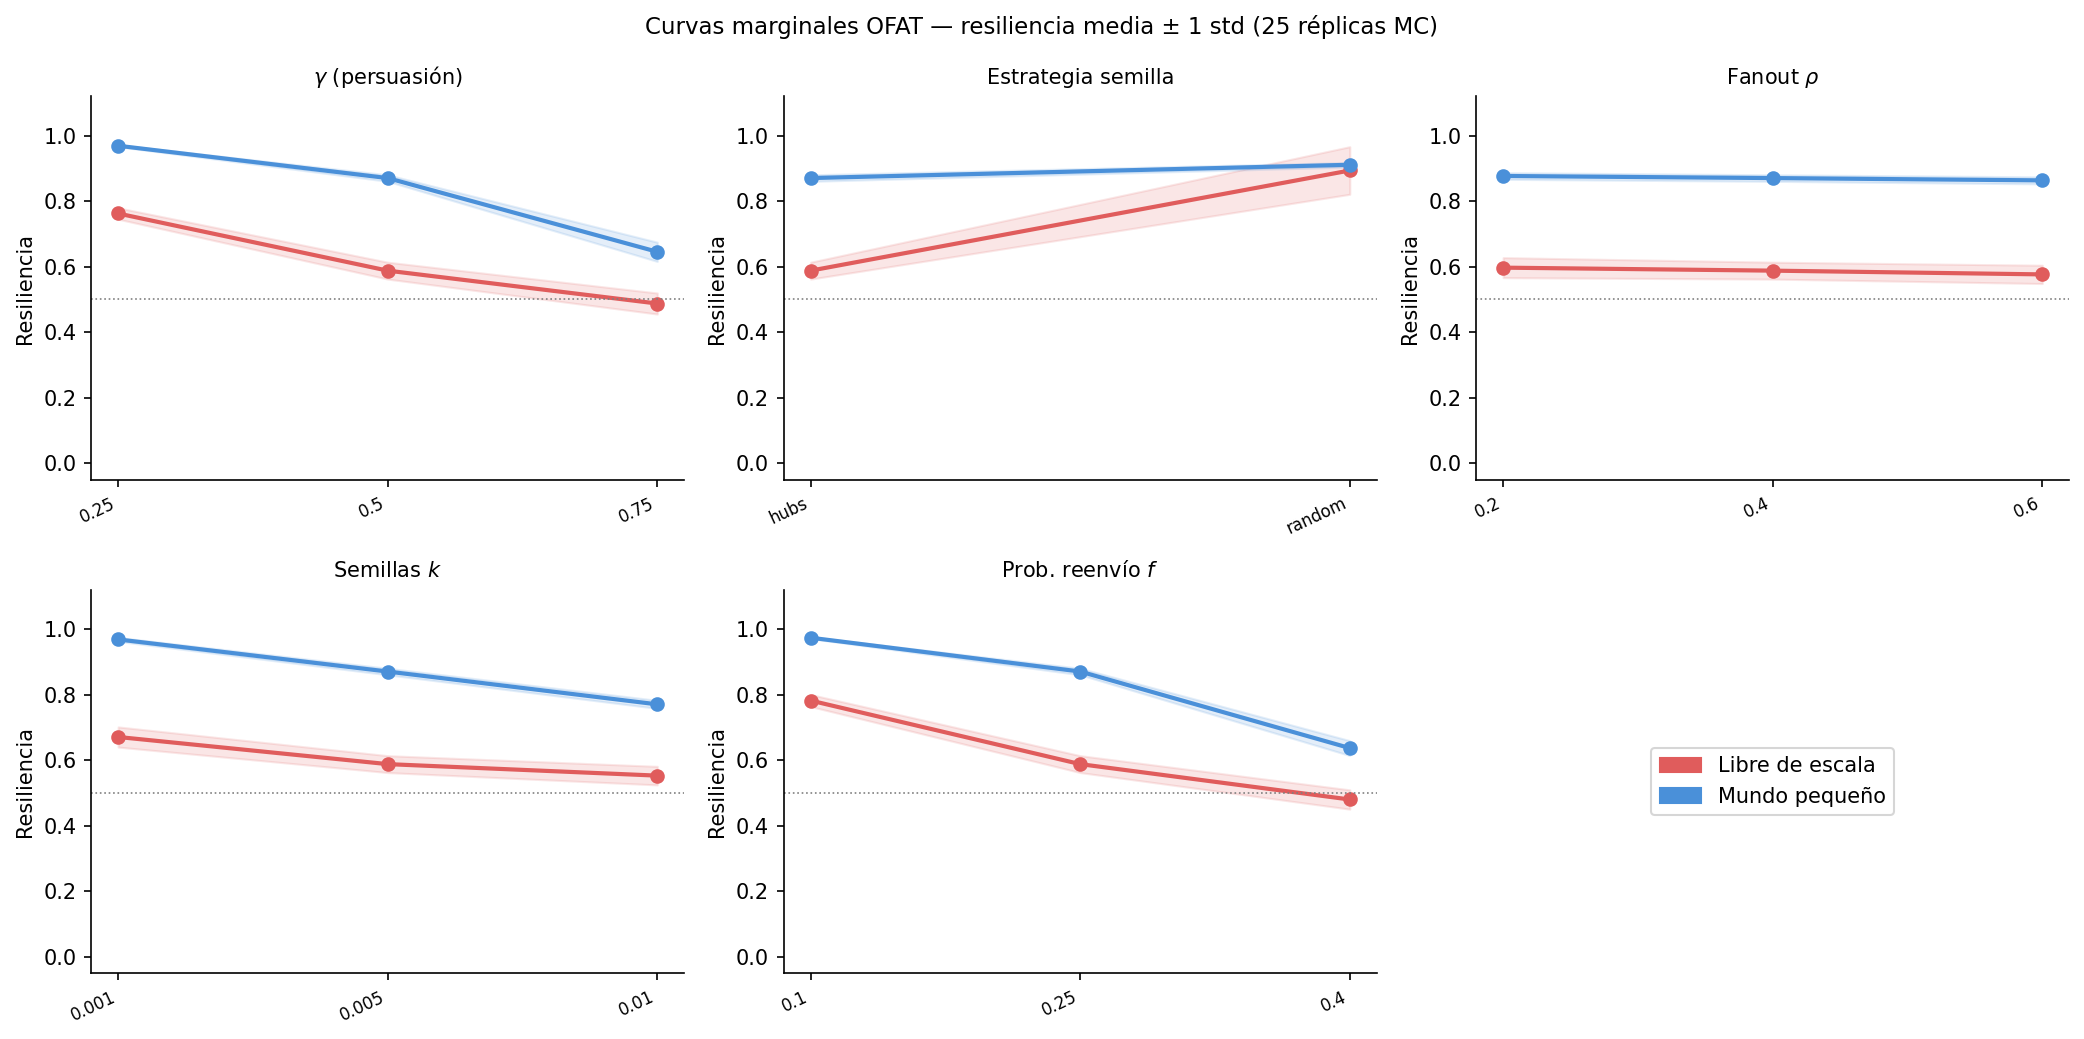
\includegraphics[width=\linewidth]{images/sweep_marginal_resiliencia.png}
    \caption{Curvas marginales OFAT. Cada línea muestra la resiliencia media $\pm 1\sigma$ sobre 50 réplicas MC para cada nivel del factor, en la red libre de escala (rojo) y mundo pequeño (azul). La línea discontinua marca $R=0{,}5$.}
    \label{fig:marginal}
\end{figure}

La Figura~\ref{fig:marginal} resume el efecto marginal de cada factor sobre la resiliencia poblacional $R = 1 - a$. Destacan tres observaciones transversales.

\textbf{La topología es el factor estructural dominante.} Bajo la configuración de referencia, la red libre de escala presenta una resiliencia media de $0{,}482$ mientras que la de mundo pequeño alcanza $0{,}746$. La diferencia de 26 puntos porcentuales refleja que la concentración de influencia en los \emph{hubs} de la red libre de escala facilita enormemente la penetración de la narrativa. Cuando el atacante siembra en \emph{hubs}, cada semilla contagia a una fracción desproporcionada de la población en los primeros pasos, antes de que los mecanismos de refuerzo social de la red de mundo pequeño puedan activarse.

\textbf{La red de mundo pequeño es más sensible a los factores de intensidad.} En los factores $\gamma$ y $f$, la variación de la resiliencia de la red de mundo pequeño a lo largo de los niveles es mucho mayor que la de la red libre de escala: la pequeña-mundo puede ser casi invulnerable ($R \approx 0{,}95$) con parámetros bajos o casi colapsada ($R \approx 0{,}31$) con parámetros altos. Esto indica que la red de mundo pequeño tiene un punto de inflexión más pronunciado, coherente con la ventana de cascada descrita por Watts~\cite{Watts2002}.

\textbf{El fanout inicial $\rho$ tiene impacto marginal.} En ambas topologías, variar el fanout de $0{,}2$ a $0{,}6$ apenas mueve la resiliencia (variación de menos de 5 puntos porcentuales), lo que indica que una vez lanzada la narrativa con al menos un 20\% de contactos iniciales, la dinámica posterior de reenvío domina sobre el arranque.

\subsection{Efecto de la ganancia de persuasión y la probabilidad de reenvío}

\begin{figure}[h!]
    \centering
    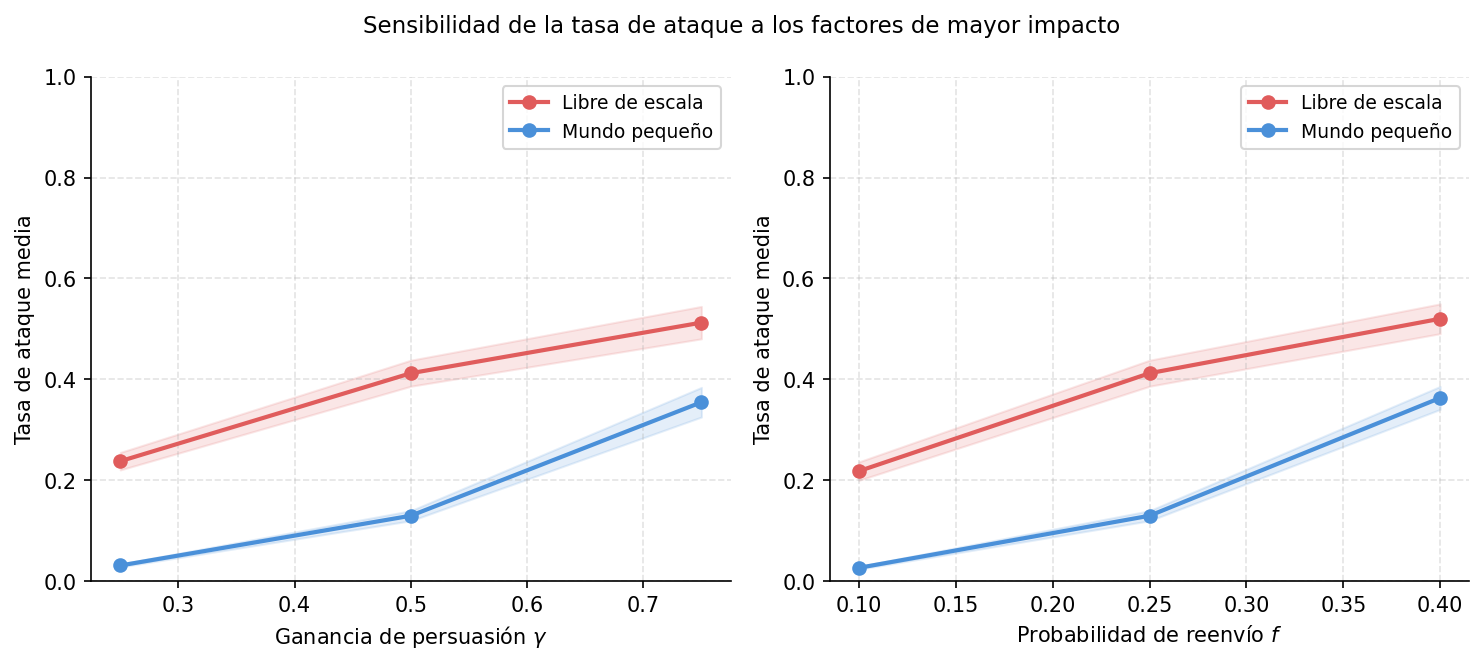
\includegraphics[width=0.9\linewidth]{images/sweep_gamma_fwd.png}
    \caption{Sensibilidad de la tasa de ataque a $\gamma$ (izquierda) y a $f$ (derecha). Las bandas sombreadas representan $\pm 1\sigma$ sobre 50 réplicas MC. La red de mundo pequeño exhibe un punto de inflexión más pronunciado que evidencia el umbral de cascada.}
    \label{fig:gammafwd}
\end{figure}

La Figura~\ref{fig:gammafwd} muestra la respuesta de ambas topologías ante los dos factores de mayor sensibilidad. La \textbf{ganancia de persuasión} $\gamma$ cuantifica el incremento de convicción por unidad de carga emocional del mensaje: a $\gamma = 0{,}25$, la red libre de escala alcanza una tasa de ataque media de $0{,}32$ mientras que la pequeña-mundo se queda en $0{,}05$; a $\gamma = 0{,}75$, ambas convergen en torno a $0{,}59$--$0{,}69$. El cruce de las curvas sugiere que redes estructuralmente más resistentes (pequeña-mundo) son más sensibles a la intensidad de la persuasión una vez superado un umbral crítico.

La \textbf{probabilidad de reenvío} $f$ muestra un patrón casi idéntico: la red de mundo pequeño pasa de una tasa de ataque de $0{,}046$ con $f = 0{,}10$ a $0{,}688$ con $f = 0{,}40$, con una aceleración especialmente pronunciada entre $f = 0{,}25$ y $f = 0{,}40$. Esta no-linealidad es la huella de la ventana de cascada: por debajo del umbral, el contagio percolativo no puede sostenerse; por encima, la red casi colapsa. En la red libre de escala la respuesta es más gradual porque los \emph{hubs} ya garantizan un nivel alto de difusión incluso con reenvío moderado.

\subsection{Vulnerabilidad estructural: siembra en hubs frente a aleatoria}

\begin{figure}[h!]
    \centering
    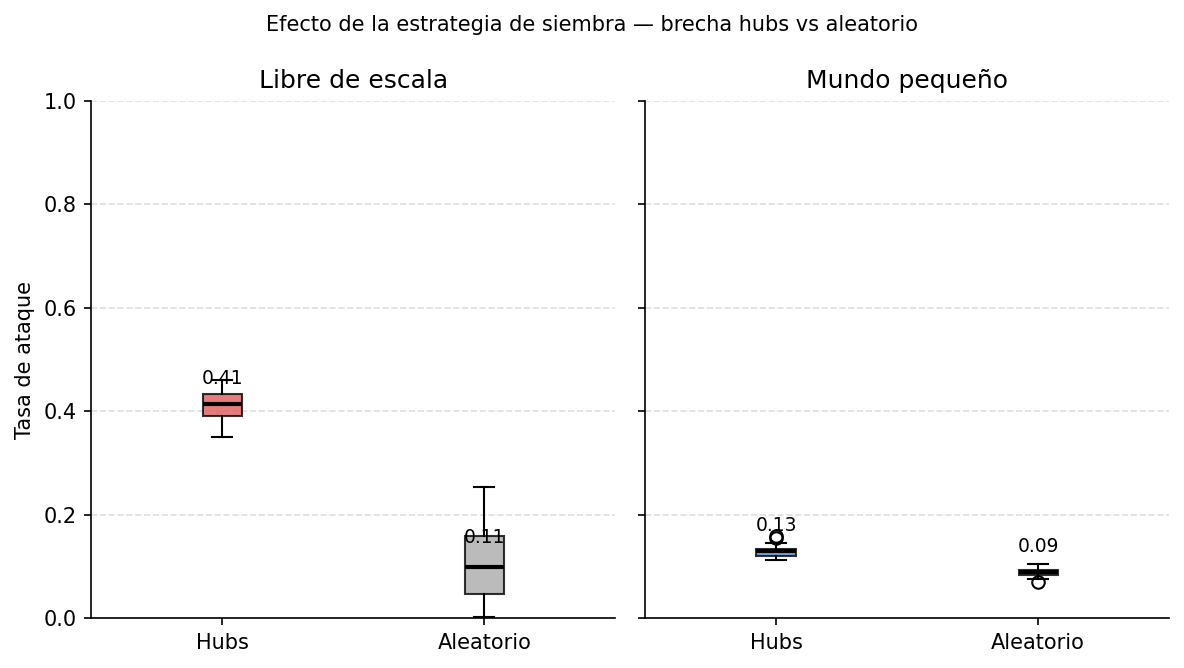
\includegraphics[width=0.75\linewidth]{images/sweep_hubs_vs_random.png}
    \caption{Distribución de la tasa de ataque según estrategia de siembra, para cada topología. Los números sobre los bigotes indican la media. La ventaja de sembrar en \emph{hubs} es mucho mayor en la red libre de escala.}
    \label{fig:hubsrandom}
\end{figure}

La Figura~\ref{fig:hubsrandom} cuantifica la vulnerabilidad estructural de cada topología. En la red libre de escala, sembrar en los 25 \emph{hubs} de mayor in-grado produce una tasa de ataque media de $0{,}518 \pm 0{,}045$ frente a $0{,}163 \pm 0{,}123$ con siembra aleatoria: una \textbf{brecha de 35 puntos porcentuales}. La alta varianza de la siembra aleatoria en escala libre refleja la dependencia de los resultados con la muestra de nodos elegidos: ocasionalmente se seleccionan nodos bien conectados por azar, con efectos similares a los \emph{hubs}.

En la red de mundo pequeño, la brecha es mucho menor ($0{,}254$ vs $0{,}171$, diferencia de 8 puntos porcentuales) y la varianza es comparable en ambas estrategias. Este resultado confirma teóricamente el resultado de Kempe, Kleinberg y Tardos~\cite{KempeKleinbergTardos2003}: la ventaja del sembrado óptimo es mayor en redes con hubs prominentes, y prácticamente se anula en redes con distribución de grado más homogénea.

\subsection{Efecto del número de semillas}

\begin{figure}[h!]
    \centering
    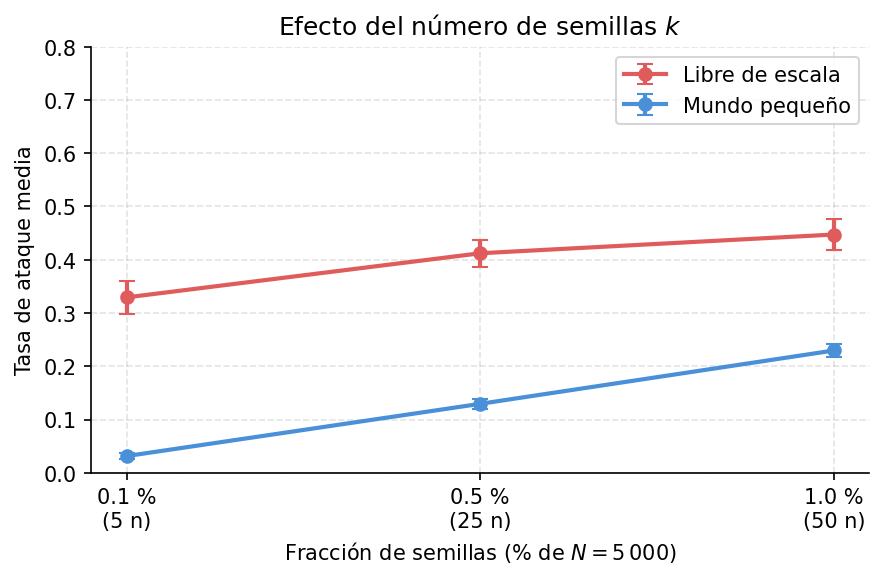
\includegraphics[width=0.6\linewidth]{images/sweep_k_seeds.png}
    \caption{Tasa de ataque media $\pm 1\sigma$ en función del número de semillas expresado como fracción de $N = 10\,000$. La red de mundo pequeño muestra mayor sensibilidad: triplicar semillas multiplica por seis la penetración.}
    \label{fig:kseeds}
\end{figure}

La Figura~\ref{fig:kseeds} muestra que el número de semillas tiene un efecto moderado pero no despreciable. En la red de mundo pequeño, el impacto es más pronunciado: pasar de 5 semillas ($0{,}1\%$) a 50 ($1\%$) incrementa la tasa de ataque de $0{,}067$ a $0{,}416$, un factor de $6\times$. En la red libre de escala el efecto es menor ($0{,}430 \to 0{,}547$) porque el \emph{hub} de arranque ya captura la mayoría del potencial de propagación con pocos nodos iniciales.

El resultado es coherente con el modelo de maximización de influencia: en redes de mundo pequeño, donde no hay \emph{hubs} que capitalicen el efecto de siembra, el número de semillas es más determinante para alcanzar la masa crítica que desencadena la cascada. En redes libre de escala, la calidad de la semilla (centralidad del nodo) domina sobre la cantidad.

\subsection{Síntesis: ranking de factores}

La Tabla~\ref{tab:ranking} ordena los cinco factores por su rango de variación de la tasa de ataque a lo largo del barrido, como medida del impacto marginal.

\begin{table}[ht]
    \centering
    \small
    \caption{Ranking de factores por impacto sobre la tasa de ataque. El rango es la diferencia entre el nivel máximo y mínimo de tasa de ataque media.}
    \label{tab:ranking}
    \begin{tabular}{@{}l cc cc@{}}
        \toprule
        & \multicolumn{2}{c}{\textbf{Libre de escala}} & \multicolumn{2}{c}{\textbf{Mundo pequeño}} \\
        \cmidrule(lr){2-3} \cmidrule(lr){4-5}
        \textbf{Factor} & Mín $a$ & Máx $a$ & Mín $a$ & Máx $a$ \\
        \midrule
        Estrategia semilla & $0{,}163$ & $0{,}518$ & $0{,}171$ & $0{,}254$ \\
        Ganancia $\gamma$ & $0{,}316$ & $0{,}594$ & $0{,}052$ & $0{,}686$ \\
        Prob.\ reenvío $f$ & $0{,}289$ & $0{,}605$ & $0{,}046$ & $0{,}688$ \\
        Semillas $k$ & $0{,}430$ & $0{,}547$ & $0{,}067$ & $0{,}416$ \\
        Fanout $\rho$ & $0{,}491$ & $0{,}524$ & $0{,}235$ & $0{,}260$ \\
        \bottomrule
    \end{tabular}
\end{table}

La estrategia de siembra tiene el mayor rango en la red libre de escala (35 pp), mientras que $\gamma$ y $f$ dominan en la red de mundo pequeño (64 y 64 pp respectivamente). El fanout es el factor de menor impacto en ambas topologías: una vez que la narrativa alcanza un mínimo de vecinos en el arranque, la dinámica posterior es independiente de ese parámetro.

\newpage

%%%%%%%%%%%%%%%%%%%%%%%%%%%%%%%%%%%%%%%%%%%%%%%%%%%%%%%%
%%%% Conclusiones %%%%%%%%%%%%%%%%%%%%%%%%%%%%%%%%%%%%%%%
%%%%%%%%%%%%%%%%%%%%%%%%%%%%%%%%%%%%%%%%%%%%%%%%%%%%%%%%
\section{Conclusiones y Trabajo Futuro}\label{sec:conclusion}

\subsection{Conclusiones}

Este trabajo ha diseñado, implementado y evaluado un simulador multiagente de propagación de narrativas sobre redes complejas orientado a medir la resistencia cognitiva de una población. Los resultados del barrido OFAT de 1\,000 corridas ($N=10\,000$, 50 réplicas MC, 7 factores) permiten extraer las siguientes conclusiones.

\textbf{C1. La topología es el factor de resiliencia más robusto.} Bajo condiciones de referencia, la red de mundo pequeño exhibe una resiliencia de $0{,}746$ frente a $0{,}482$ de la red libre de escala, una diferencia que se mantiene estable a lo largo de todos los factores analizados. La arquitectura de la red no es un factor controlable por el defensor en el corto plazo ---la sociedad está organizada como está--- pero sí indica dónde es más urgente invertir en resiliencia: las plataformas digitales libre de escala son estructuralmente más vulnerables que las redes de relaciones presenciales.

\textbf{C2. La ganancia de persuasión y la viralidad son los factores más palancables por el atacante.} Los parámetros $\gamma$ (intensidad de la persuasión emocional) y $f$ (probabilidad de reenvío) controlan si la narrativa permanece confinada o desencadena una cascada global, especialmente en la red de mundo pequeño donde el punto de inflexión es pronunciado. Desde la perspectiva defensiva, estos resultados sugieren que las intervenciones más eficaces son las que reducen la carga emocional de la narrativa (verificación rápida, contra-narrativa que desactiva la emoción) y las que frenan el reenvío (reducción algorítmica de la amplificación viral).

\textbf{C3. La ventaja del sembrado en hubs es cuantificable y asimétrica.} En la red libre de escala, el atacante que selecciona los 25 nodos de mayor in-grado obtiene una penetración tres veces superior a la de un atacante que siembra aleatoriamente ($0{,}518$ vs $0{,}163$). Esta asimetría es la expresión operativa del resultado de Kempe, Kleinberg y Tardos~\cite{KempeKleinbergTardos2003}: el problema de maximización de influencia tiene solución práctica en redes con \emph{hubs}, y el atacante que la explota tiene una ventaja estructural enorme. Desde la óptica defensiva, esto señala a los \emph{hubs} como los nodos cuya resiliencia individual (umbral $\theta_i$ alto) tiene mayor impacto sobre la resistencia colectiva.

\textbf{C4. El fanout inicial es irrelevante una vez superado el umbral mínimo de arranque.} La variación del fanout de $0{,}2$ a $0{,}6$ no produce diferencias estadísticamente significativas en la tasa de ataque. Este resultado simplifica la modelización: no es necesario calibrar con precisión el comportamiento de publicación inicial del atacante; lo que importa es si la narrativa alcanza la masa crítica en los primeros pasos.

\textbf{C5. Las métricas implementadas operacionalizan el concepto de superioridad cognitiva de la OTAN.} La tasa de ataque $a$, la resiliencia $R$, la entropía cognitiva $H$ y el tiempo de penetración $t_{50}$ traducen una definición cualitativa ---"luchar por la superioridad cognitiva"~\cite{NATOChiefScientist2025}--- en magnitudes medibles y comparables entre condiciones experimentales. La entropía cognitiva, en particular, captura el colapso de la diversidad de creencias que el \emph{Cognitive Net Assessment}~\cite{PolytechniqueCNA2026} identifica como la consecuencia más duradera de una operación cognitiva exitosa.

\subsection{Trabajo Futuro}

Las líneas de trabajo futuro más relevantes son:

\begin{itemize}
    \item \textbf{Agente cognitivo-emocional.} Implementar el experimento completo con \texttt{BayesianAgent}: el cerebro emocional vectorial de 11 dimensiones está diseñado pero no evaluado. Su inclusión permitiría estudiar cómo la composición emocional de la narrativa (miedo, ira, sorpresa) modula la resistencia de forma diferencial respecto al modelo de umbral escalar.

    \item \textbf{Redes reales.} Descargar grafos de SNAP (ego-Facebook, Twitter) y ejecutar el mismo barrido OFAT para contrastar si las propiedades de las redes sintéticas son representativas. Las redes reales presentan estructura comunitaria y correlaciones de grado que pueden generar dinámicas de cascada cualitativamente distintas.

    \item \textbf{Capa multicapa analógico-digital.} El simulador está preparado para operar con grafos multicapa pero los experimentos solo han usado capas monolayer. Activar la capa analógica (mundo pequeño) y la digital (libre de escala) en paralelo permitiría modelar cómo la desinformación cruza de una capa a otra y si la resiliencia de la capa analógica actúa como cortafuegos.

    \item \textbf{Contramedidas de resiliencia.} Estudiar intervenciones defensivas cuantificando su eficacia en el mismo marco: vacunación topológica (aumentar $\theta_i$ de los \emph{hubs}), inyección de contra-narrativa (semillas con veracidad alta) y reducción algorítmica del reenvío. El simulador es directamente extensible para estos experimentos sin modificar su arquitectura.

    \item \textbf{Horizonte temporal corto.} Los experimentos actuales operan en el horizonte largo plazo (estabilización de la cascada). Estudiar métricas de corto plazo ---velocidad de penetración inicial, tiempo de respuesta defensiva óptima--- requeriría análisis de las trazas a resolución fina en los primeros 5--10 pasos de simulación.
\end{itemize}

\newpage

%%%%%%%%%%%%%%%%%%%%%%%%%%%%%%%%%%%%%%%%%%%%%%%%%%%%%%%%
%%%% Referencias %%%%%%%%%%%%%%%%%%%%%%%%%%%%%%%%%%%%%%%
%%%%%%%%%%%%%%%%%%%%%%%%%%%%%%%%%%%%%%%%%%%%%%%%%%%%%%%%
\section{Bibliograf\'ia} \label{sec:bibliography}

\printbibliography[heading=none]

\end{refsection}
\newpage

%%%%%%%%%%%%%%%%%%%%%%%%%%%%%%%%%%%%%%%%%%%%%%%%%%%%%%%%
%%%% Anexos %%%%%%%%%%%%%%%%%%%%%%%%%%%%%%%%%%%%%%%%%%%%
%%%%%%%%%%%%%%%%%%%%%%%%%%%%%%%%%%%%%%%%%%%%%%%%%%%%%%%%
\appendix
\section{T\'itulo del Anexo A}
\textcolor{red}{Incluye cuantos anexos sean necesarios. El objetivo de los anexos es incluir informaci\'on importante pero demasiado extensa para incluir en el texto del proyecto (p.ej., gr\'aficas extra o tablas completas de experimentos/hiperpar\'ametros. Pregunta a tu director cuando no est\'es seguro.}

\end{document}




